%% 
%% Copyright 2007, 2008, 2009 Elsevier Ltd
%% 
%% This file is part of the 'Elsarticle Bundle'.
%% ---------------------------------------------
%% 
%% It may be distributed under the conditions of the LaTeX Project Public
%% License, either version 1.2 of this license or (at your option) any
%% later version.  The latest version of this license is in
%%    http://www.latex-project.org/lppl.txt
%% and version 1.2 or later is part of all distributions of LaTeX
%% version 1999/12/01 or later.
%% 
%% The list of all files belonging to the 'Elsarticle Bundle' is
%% given in the file `manifest.txt'.
%% 

%% Template article for Elsevier's document class `elsarticle'
%% with numbered style bibliographic references
%% SP 2008/03/01

\documentclass[preprint,12pt]{elsarticle}

\usepackage{graphicx} 	  %% The graphicx package provides the includegraphics command.
\usepackage{amssymb} 	%% The amssymb package provides various useful mathematical symbols

\usepackage{color}
\usepackage{amsmath}
\usepackage{mathtools}
\usepackage{fullpage}
\usepackage{algorithmic}
\DeclareMathOperator*{\argmin}{argmin}
\DeclareMathOperator*{\argmax}{argmax}
\algsetup{linenosize=\small}
\usepackage[table,xcdraw]{xcolor}
\usepackage{multirow}
\usepackage[super]{nth}
\usepackage{graphicx,adjustbox}
\usepackage{caption}
\usepackage[labelformat=simple]{subcaption}
\usepackage{comment}
\usepackage{setspace}
\usepackage{textcomp}
\usepackage{xspace}
\usepackage{siunitx}
\usepackage{epsfig}
\usepackage{epstopdf}
\usepackage{soul}
\usepackage{url}
\usepackage{tablefootnote}
\DeclareMathOperator{\E}{\mathbb{E}} % Expectation Symbol
\usepackage[linesnumbered,ruled]{algorithm2e}
\usepackage{booktabs}
\usepackage{hyperref}
\usepackage[normalem]{ulem}
\usepackage{footnote}
\usepackage[misc,geometry]{ifsym} 
\makesavenoteenv{tabular}

%% Other
\DeclarePairedDelimiter\abs{\lvert}{\rvert}

\renewcommand\thesubfigure{(\alph{subfigure})}
\let\OldTexttrademark\texttrademark
\renewcommand{\texttrademark}{\OldTexttrademark\xspace}%
\DeclarePairedDelimiter\ceil{\lceil}{\rceil}
%% Use the options 1p,twocolumn; 3p; 3p,twocolumn; 5p; or 5p,twocolumn
%% for a journal layout:
%% \documentclass[final,1p,times]{elsarticle}
%% \documentclass[final,1p,times,twocolumn]{elsarticle}
%% \documentclass[final,3p,times]{elsarticle}
%% \documentclass[final,3p,times,twocolumn]{elsarticle}
%% \documentclass[final,5p,times]{elsarticle}
%% \documentclass[final,5p,times,twocolumn]{elsarticle}

%\usepackage{authblk}

%% Use the option review to obtain double line spacing
%% \documentclass[authoryear,preprint,review,12pt]{elsarticle}

%% Use the options 1p,twocolumn; 3p; 3p,twocolumn; 5p; or 5p,twocolumn
%% for a journal layout:
%% \documentclass[final,1p,times]{elsarticle}
%% \documentclass[final,1p,times,twocolumn]{elsarticle}
%% \documentclass[final,3p,times]{elsarticle}
%% \documentclass[final,3p,times,twocolumn]{elsarticle}
%% \documentclass[final,5p,times]{elsarticle}
%% \documentclass[final,5p,times,twocolumn]{elsarticle}

%% For including figures, graphicx.sty has been loaded in
%% elsarticle.cls. If you prefer to use the old commands
%% please give \usepackage{epsfig}
\usepackage{epsfig}
%% The amssymb package provides various useful mathematical symbols
\usepackage{amssymb}
%% The amsthm package provides extended theorem environments
%% \usepackage{amsthm}
\newcommand{\francesc}[1]{\textcolor{blue}{#1}}
\newcommand{\francesco}[1]{\textcolor{orange}{#1}}
%% The lineno packages adds line numbers. Start line numbering with
%% \begin{linenumbers}, end it with \end{linenumbers}. Or switch it on
%% for the whole article with \linenumbers.
%% \usepackage{lineno}

\journal{Computer Networks}

\begin{document}

\begin{frontmatter}

%% Title, authors and addresses

%% use the tnoteref command within \title for footnotes;
%% use the tnotetext command for theassociated footnote;
%% use the fnref command within \author or \address for footnotes;
%% use the fntext command for theassociated footnote;
%% use the corref command within \author for corresponding author footnotes;
%% use the cortext command for theassociated footnote;
%% use the ead command for the email address,
%% and the form \ead[url] for the home page:
%% \title{Title\tnoteref{label1}}
%% \tnotetext[label1]{}
%% \author{Name\corref{cor1}\fnref{label2}}
%% \ead{email address}
%% \ead[url]{home page}
%% \fntext[label2]{}
%% \cortext[cor1]{}
%% \address{Address\fnref{label3}}
%% \fntext[label3]{}

\title{Collaborative Spatial Reuse in Wireless Networks via Selfish Multi-Armed Bandits}

\author[label1, label4]{Francesc Wilhelmi}\ead{francisco.wilhelmi@upf.edu}
\author[label2]{Cristina~Cano}
\author[label3]{Gergely~Neu}
\author[label1]{Boris~Bellalta} 
\author[label3]{Anders~Jonsson}
\author[label1]{Sergio~Barrachina-Mu\~noz}
\address[label1]{Wireless Networking Research Group (WN-UPF), 08002 Barcelona, Spain}
\address[label2]{Wireless Networks Research Group (WINE-UOC), 08860 Castelldefels (Barelona), Spain}
\address[label3]{Artificial Intelligence and Machine Learning Research Group (AIML-UPF), 08002 Barcelona, Spain}

\begin{abstract}
Next-generation wireless deployments are characterized by being dense and uncoordinated, which often leads to inefficient use of resources and poor performance. To solve this, we envision the utilization of completely decentralized mechanisms to enable Spatial Reuse (SR). In particular, we concentrate in Reinforcement Learning (RL), and more specifically, in Multi-Armed Bandits (MABs), to allow networks to modify both their transmission power and channel based on their experienced throughput. In this work, we study the exploration-exploitation trade-off by means of the $\varepsilon$-greedy, EXP3, UCB and Thompson sampling action-selection strategies. Our results show that optimal proportional fairness can be achieved, even if no information about neighboring networks is available to the learners and WNs operate selfishly. However, there is high temporal variability in the throughput experienced by the individual networks, specially for $\varepsilon$-greedy and EXP3. We identify the cause of this variability to be the adversarial setting of our setup in which the set of most played actions provide intermittent good/poor performance depending on the neighboring decisions. We also show that this variability is reduced using UCB and Thompson sampling, which are parameter-free policies that perform exploration according to the reward distribution of each action.
\end{abstract}

\begin{keyword}
High-Density Wireless Networks, Interference, Decentralized learning, Multi Armed Bandits, Spatial Reuse, Resource Allocation.
\end{keyword}

\end{frontmatter}

%\vfill
%Francesc Wilhelmi (e-mail \href{francisco.wilhelmi@upf.edu}{francisco.wilhelmi@upf.edu}), Sergio Barrachina-Mu\~noz and Boris Bellalta are with the Wireless Networking Research Group, Universitat Pompeu Fabra, 08002 Barcelona, Spain. Cristina Cano is with the Wireless Networks Research Group, Universitat Oberta de Catalunya (UOC), 08860 Castelldefels (Barelona), Spain. Anders~Jonsson and Gergely~Neu are with the Artificial Intelligence and Machine Learning Research Group, Universitat Pompeu Fabra (UPF), 08002 Barcelona, Spain.

\newpage
%% \linenumbers

%%%%%%%%%%%%%%%%%%%%%%%
%%%  I. INTRODUCTION 
%%%%%%%%%%%%%%%%%%%%%%%
\section{Introduction}
\label{section:introduction}
Due to the growing popularity of wireless deployments, especially the ones based on the IEEE 802.11 standard (i.e., Wi-Fi), it is very common to find independent overlapping Wireless Networks (WNs) sharing the same channel resources. Due to the decentralized nature of such kind of deployments, the lack of organization and/or agreement on sharing policies leads to inefficient resources allocation, both in spectral and spatial domains. An illustrative example about the inefficiency noticed in WNs regarding channel sharing can be found in \cite{akella2007self}, where the authors show that the power level used by wireless devices is typically set, by default, to the maximum, regardless of the distance between communicating nodes, and of the channel occupancy \cite{akella2007self}. In decentralized environments, providing a model to obtain the optimal solution can be extremely complex. In WNs, the interactions between devices depend on many features (such as position, environment, transmit power) and are hard to derive. On top of this, network dynamics, in terms of user arrivals and departures, makes the resource allocation problem even harder. 

In order to address the SR problem in decentralized WNs, we focus attention on Reinforcement Learning (RL), which has recently become very popular to solve many well-known problems in wireless communications. Some examples can be found for packet routing \cite{littman1993distributed}, Access Point (AP) selection \cite{bojovic2011supervised, bojovic2012neural}, optimal rate sampling \cite{combes2014optimal}, or energy harvesting in heterogeneous networks \cite{miozzo2015distributed}. Using online learning, a learner (or agent) obtains data in a sequential order and uses it to predict future good-performing actions. Online learning is, therefore, useful to cope with complex and dynamic environments. This background encourages us to approach a solution for the decentralized SR problem in WNs through online learning techniques. In particular, we exploit dynamic channel selection and transmit power adjustment for dealing with the performance issues resulting from uncoordinated resource sharing in WNs. While a proper frequency planning allows to reduce the interference between wireless devices, tuning the transmit power adds an extra level of SR that can result in improved throughput and fairness.

From the family of online algorithms, we propose the utilization of Multi-Armed Bandits (MABs) \cite{BCB12}, which is a well-known model in the online learning literature for solving resource allocation problems. In MABs, a given agent seeks to learn a hidden reward distribution while maximizing the gains. This is known as the exploration-exploitation trade-off. %(exploitation focuses on obtaining the maximum instantaneous reward, while exploration aims to maximize the long-term reward)	
While exploitation selects actions with the goal of maximizing long-term reward given the current estimate, exploration selects actions with the goal of improving the estimate. Unlike for classical RL, MABs do not consider states\footnote{A state refers to a particular situation experienced by a given agent, which is defined by a set of conditions. By having an accurate knowledge on its current situation, an agent can define state-specific strategies that maximize its profits.} in general, which can be hard to define for the decentralized SR problem. On the one hand, spatial interference cannot be binary treated, thus leading to complex interactions between nodes. On the other hand, the adversarial setting unleashed by decentralized deployments increases the system complexity, since the state not only depends on the actions taken by a given node, but also on the adversaries behavior.

This work extends our previous results presented in \cite{wilhelmi2017implications}, which were obtained by applying a stateless variation of Q-learning to the SR problem in WNs. Here we generalize the contributions done by implementing several action-selection strategies to allow WNs choose the channel and transmit power to use based on the resulting performance. In this paper, then, we provide a tutorial-based application of MABs to the decentralized SR problem, in order to maximize performance while observing the result from using different SR settings. According to that, we aim to illustrate the main benefits and drawbacks of applying different well-known learning techniques in a selfish way, i.e., independent WNs base their strategy on their own experienced performance. On the one hand, we evaluate the impact of varying parameters intrinsic to the proposed algorithms on the resulting throughput and fairness. In addition, we analyze the effects of learning selfishly, in order to shed some light on the future of decentralized approaches. Notably, we observe that even though players act selfishly, there are algorithms %learn to play collaborative actions
learn to play actions that enhance the overall performance, some times at the cost of high temporal variability. Considering selfish WNs and still obtaining collaborative behaviors is appealing to typical chaotic and dynamic deployments as we get rid of the need for message passing, or inference of neighboring conditions. 

The main contributions of this work are summarized below:
\begin{itemize}		
	\item We devise the feasibility of applying MAB algorithms as defined in the online learning literature to solve the resource allocation problem in WNs.
	\item We study the impact of different parameters intrinsic to the action-selection strategies considered (e.g., exploration coefficients, learning rates) on network performance.
	\item We show that there are algorithms learn to play collaborative actions even though the WNs act selfishly, which is appealing to practical application in chaotic and dynamic environments. In addition, we shed some light on the root causes of this phenomena. 
\end{itemize}

The remaining of this document is structured as follows: Section \ref{section:related_work} outlines relevant related work. Section \ref{section:mabs} introduces the proposed learning algorithms and their practical implementation for the resource allocation problem in WNs. Then, Section \ref{section:system_model} presents the simulation scenarios and the considerations taken into account. The simulation results are later presented in Section \ref{section:performance_evaluation}. Finally, Section \ref{section:conclusions} provides some final remarks.
	
%%%%%%%%%%%%%%%%%%%%%%%
%%%  II. RELATED WORK 
%%%%%%%%%%%%%%%%%%%%%%%
\section{Related Work}
\label{section:related_work} 		
In this paper we approach the decentralized SR problem through Dynamic Channel Allocation (DCA) and Transmit Power Control (TPC). While the former aims to allocate the available frequency range among potentially overlapping WNs, the latter attempts to increase the number of parallel transmissions by adjusting the power transmitted by each WN. While DCA operates at the frequency level, TPC deals with more complex spatial interactions. For that, an approach that dynamically tunes the transmit power may severely affect higher communication layers such as network (routing) or transport (congestion). TPC directly affects the transmission range, the data rate and the energy consumption, and it may create unidirectional links that unleash fairness issues. In fact, acknowledgments (ACKs) and RTS/CTS frames assume bidirectionality. 

DCA has been extensively exploited from the centralized perspective, especially through techniques based on graph coloring \cite{riihijarvi2005frequency, mishra2005weighted}. Despite these kind of approaches allow to effectively reduce the interference between WNs, a certain degree of communication is required. Regarding decentralized methods, the authors in \cite{akl2007dynamic} propose a very simple approach in which each AP maintains an interference map of their neighbors, so that channel assignment is done through interference minimization. Unfortunately, the interactions between APs due to decentralization are not studied. Separately, \cite{chen2007improved} proposes two decentralized approaches that rely in the interference measured at both APs and STAs to calculate the best frequency channels for dynamic channel allocation. To do so, a WN, in addition to the interference sensed by its associated devices, considers other metrics such as the amount of traffic, so that some kind of coordination is required at the neighbor level (periodic reporting). 

For the case of TPC, one of the first works in studying power management is \cite{elbatt2000power}, which shows that large improvements can be achieved if selecting the appropriate transmit power level in ad-hoc WNs. A centralized approach for TPC is presented in \cite{tang2014joint}, which performs power control and Rate Adaptation (RA) in subgroups of Wireless Local Area Networks (WLANs). The creation of clusters allows defining independent power levels between devices in the same group, which are useful to avoid asymmetric links. However, to represent all the possible combinations, graphs can become very large, specially in high-density deployments. Furthermore, we find a decentralized approach that relies on real-time channel measurements \cite{gandarillas2014dynamic}. The proposed mechanism (so called Dynamic Transmission Power Control) is based on a set of triggered thresholds that increase/decrease the transmit power according to the situation. The main problem is that thresholds are set empirically (based on simulations), so the mechanism may not always improve performance.

%------------------------
% Decentralised Learning: Previous work
%------------------------
\subsection{Solving WNs Resource Allocation Problems via Bandits}
\label{section:previous_work}
In the online learning literature, several MAB settings have been considered such as stochastic bandits \cite{thompson1933likelihood,lai1985asymptotically,auer2002finite}, adversarial bandits \cite{auer1995gambling,auer2002nonstochastic}, restless bandits \cite{whittle1988restless}, contextual bandits \cite{LCLS10} and linear bandits \cite{abe2003reinforcement,APS11}, and numerous exploration-exploitation strategies have been proposed such as \textit{$\varepsilon$-greedy} \cite{sutton1998reinforcement,auer2002finite}, \textit{upper confidence bound} (UCB) \cite{lai1985asymptotically,Agr95,BuKa96,auer2002finite}, \textit{exponential weight algorithm for exploration and exploitation} (EXP3) \cite{auer1995gambling,auer2002finite} and \textit{Thompson sampling} \cite{thompson1933likelihood}. The classical multi-armed bandit problem models a sequential interaction scheme between a learner and an environment. The learner sequentially selects one out of $K$ actions (often called \emph{arms} in this context) and earns some rewards determined by the chosen action and also influenced by the environment. Formally, the problem 
is defined as a repeated game where the following steps are repeated in each round $t=1,2,\dots,T$:
\begin{enumerate}
	\item The environment fixes an assignment of rewards $r_{a,t}$ for each action $a\in[K] \stackrel{\text{def}}{=} \left\{1,2,\dots,K\right\}$,
	\item the learner chooses action $a_t\in[K]$,
	\item the learner obtains and observes reward $r_{a_t,t}$.
\end{enumerate}
The bandit literature largely focuses on the perspective of the learner with the objective of coming up with learning algorithms that attempt to maximize the sum of the rewards gathered during the whole procedure (either with finite or infinite horizon). As noted above, this problem has been studied under various assumptions made on the environment and the structure of the arms. The most important basic cases are the \emph{stochastic} bandit problem where, for each particular arm $a$, the rewards are i.i.d.~realizations of random variables from a fixed (but unknown) distribution $\nu_a$, and the \emph{non-stochastic} (or \emph{adversarial}) bandit problem where the rewards are chosen arbitrarily by the environment. In both cases, the main challenge for the learner is the \emph{partial observability} of the rewards: the learner only gets to observe the reward associated with the chosen action $a_t$, but never observes the rewards realized for the other actions.

Let ${\rm r}_{a^*,t}$ and ${\rm r}_{a,t}$ be the rewards obtained at time $t$ from choosing actions $a^*$ (optimal) and $a$, respectively. Then, the performance of learning algorithms is typically measured by the \emph{total expected regret} defined as  \[R_T = \sum_{t=0}^{T} \mathbb{E}\left[\left({\rm r}_{a^*,t} - {\rm r}_{a,t}\right)\right].\]

An algorithm is said to \emph{learn} if it guarantees that the regret grows sublinearly in $T$, that is, if $R_T = o(T)$ is guaranteed as $T$ grows large, or, equivalently, that the average regret $R_T/T$ converges to zero. Intuitively, sublinear regret means that the learner eventually identifies the action with the highest long-term payoff. Note, as well, that the optimal action $a^*$ is the same across all the rounds. Most bandit algorithms come with some sort of a guaranteed upper bound on $R_T$ which allows for a principled comparison between various methods. 

To the best of our knowledge, there is very little related work on applying multi-armed bandit techniques to the problem of resource allocation in WNs. In \cite{coucheney2015multi}, the authors propose modeling a resource allocation problem in LTE networks through MABs. In particular, a set of Base Stations (BS) learn the best configuration of Resource Blocks (RBs) in a decentralized way. For that purpose, a variation of EXP3 (so-called Q-EXP3) is proposed, which allows to reduce the strategy set. Despite a regret bound is provided, it is subject to the fact that an optimal resource allocation exists, i.e., every BS obtains the necessary resources. In addition, a large number of iterations is required to find the optimal solution in a relatively small scenario, thus revealing the difficulties shown by decentralized settings.

More related to the problem proposed here, the authors in \cite{maghsudi2015joint} show a channel selection and power control approach in infrastructureless networks, which is modeled through bandits. In particular, two different strategies are provided to improve the performance of two Device to Device (D2D) users (each one composed by a transmitter and a receiver), which must learn the best channel and transmit power to be selected. Similarly to our problem, users do not have any knowledge on the channel or the other's configuration, so they rely on the experienced performance in order to find the best configuration. An extension of \cite{maghsudi2015joint} is provided by the same authors in \cite{maghsudi2015channel}, which includes a calibrated predictor (referred in the work as \textit{forecaster}) to infer the behavior of the other devices in order to counter act their actions. In each agent, the information of the forecaster is used to choose the highest-rewarding action with a certain probability, while the rest of actions are randomly selected. Henceforth, assuming that all the networks use a given strategy $\mathcal{X}$, fast convergence is ensured. Results show that channel resources are optimally distributed in a very short time frame through a fully decentralized algorithm that does not require any kind of coordination. Both aforementioned works rely in the existence of a unique Nash Equilibrium, which favors convergence. In contrast, in this article we aim to extend Bandits utilization to denser deployments, and, what is more important, to scenarios with limited available resources in which there is not a unique Nash Equilibrium (NE) that allows fast-convergence. Thus, we aim to capture the effects of applying selfish strategies in a decentralized way (i.e., agent $i$ follows a strategy $\mathcal{X}_i$ that does not consider the strategies of the others) and we also provide insight about the importance of past information for learning in dense WNs, which has not been studied before.

%%%%%%%%%%%%%%%%%%%%%%%%%%%%%%%
%III. MABs APPLICATION									    %	
%%%%%%%%%%%%%%%%%%%%%%%%%%%%%%%
\section{Multi-Armed Bandits for Improving Spatial Reuse in WNs}
\label{section:mabs}	
The decentralized resource allocation problem in WNs we aim to solve in this work can be modeled as an approximation of contextual bandits. Originally, the contextual bandits problem considers the existence of a context (or a state) that influences the action-selection process. As a consequence, the set of available strategies varies with the context and the probability distribution of a given reward depends both on the chosen actions and also on the context. In the resource allocation problem at hand, the context could include information such as the number of neighboring WNs, their position, their current channel selection, the transmission power they use as well as their action-selection strategies, among other. However, we are interested in the case where no context can be inferred given that such information is hard and costly to obtain in practice, especially in dynamic scenarios. Thus, we model the decentralized SR problem in WNs as an adversarial bandit problem, in which the actions of a given WN affect the pay-off distributions of the others' actions. Such model requires the existence of a NE with a pure strategy,\footnote{A pure strategy NE is conformed by a set of strategies and payoffs, so that no player can obtain further benefits by deviating from its strategy.} which does not always hold for unplanned deployments due to the scarcity of the available resources and the number of overlapping WNs. Understanding the implications derived from such an adversarial setting in the absence of a NE is one the main goals of this paper, which, to the best of our knowledge, has been barely considered in the previous literature.

We model this adversarial problem as follows. Let arm $a \in \mathcal{A}$ (we denote the size of $\mathcal{A}$ with K) be a configuration that a WN may choose. Each configuration is a combination of channel and transmit power (e.g., $a_1$ = \{Channel: 1, TPC: 5 dBm\}), and grants a reward that depends on the others' configuration. Let $\Gamma_{i,t}$ be the throughput experienced by $\text{WN}_i$ at time $t$, and $\Gamma_{i}^*$ the maximum achievable throughput by $\text{WN}_i$ in case of isolation (i.e., no interference is experienced in the selected channel). We then define the reward $r_{i,t}$ experienced by $\text{WN}_i$ at time $t$ as:

\begin{equation}
r_{i,t} = {\frac{\Gamma_{i,t}}{{\Gamma_{i}^*}}} \leq 1,
\label{eq:reward_generation}
\nonumber
\end{equation}

For simplicity, we consider that each WN is composed by an AP and a single STA, so that downlink traffic is held. Note that in typical uncoordinated wireless deployments (e.g., residential buildings), STAs are typically close to the AP to which they are associated. Thus, having several STAs associated to the same AP does not significantly impact the inter-WNs interference we study in this work. According to that, $\Gamma_{i}^*$ is computed as $B \cdot \log_{2}(1 + \text{SNR}_{i})$, where $B$ is the bandwidth, and $\text{SNR}_{i}$ is the Signal-to-Noise ratio experienced by the STA of $\text{WN}_i$. We consider this model because it allows to properly capture the interference generated between WNs, which is sought to be minimized.

We have considered the \emph{$\varepsilon$-greedy}, \emph{EXP3}, \emph{UCB} and \emph{Thompson sampling} action-selection strategies, which are described next in this section. While $\varepsilon$-greedy and EXP3 explicitly include the concepts of \emph{exploration coefficient} and \emph{learning rate}, respectively, UCB and Thompson sampling are parameter-free policies that extend the concept of exploration (actions are explored according to their estimated value and not by commitment). Henceforth, we are able to study the effects of these different kind of policies on the WNs behavior. Moreover, we chose the aforementioned policies because they are widely spread and considered of remarkable importance in the MABs literature.

Furthermore, in order to provide a fair comparison, we have considered that all the policies use the same reward. Regarding the learning process, we assume that WNs select actions during the same time slot. The reward experienced by the WNs is computed once all of them have chosen their action for the current iteration. In practice the action-selection process at WNs will most probably not be synchronized but we leave the study of any possible effects of that desynchronization to future work.

%------------------------
% Bandits - e-greedy
%------------------------
\subsection{$\varepsilon$-greedy}
\label{section:bandits_egreedy}	
The \emph{$\varepsilon$-greedy} policy \cite{sutton1998reinforcement,auer2002finite} is arguably the simplest learning algorithm attempting to deal with exploration-exploitation trade-offs. In each round $t$, the $\varepsilon$-greedy algorithm explicitly decides whether to explore or exploit: with probability $\varepsilon$, the algorithm picks an arm uniformly at random (exploration), and otherwise it plays the arm with the highest empirical return $\hat{r}_{k,t}$ (exploitation). 

In case $\varepsilon$ is fixed for the entire process, the expected regret is obviously going to grow linearly as $\Omega\left(\varepsilon T\right)$ in general. Therefore, in order to obtain a sublinear regret guarantee (and thus an asymptotically optimal growth rate for the total rewards), it is critical to properly adjust the exploration coefficient. Thus, in our implementation of the $\varepsilon$-greedy algorithm, we use a time-dependent exploration rate of $\varepsilon_t = \varepsilon_0 / \sqrt{t}$, as suggested in the literature \cite{auer2002finite}. The adaptation of this policy to our setting is shown as Algorithm \ref{alg:egreedy}.

\begin{algorithm}[H]	
	\SetAlgoLined
	\KwIn{SNR: information about the Signal-to-Noise Ratio received at the STA, $\mathcal{A}$: set of possible actions in \{$a_1, ..., a_K$\}}
	\textbf{Initialize:} $t=0$, $\varepsilon_t = \varepsilon_0$, $r_{k} = 0, \forall a_k \in \mathcal{A}$\\
	\While{active}{
		Select $a_k$  $\begin{cases}
		\underset{k=1,...,K}{\text{argmax }} r_{k,t},& \text{with prob. } 1 - \varepsilon\\
		k \sim \mathcal{U}(1, K),              & \text{otherwise}
		\end{cases}$\\
		Observe the throughput experienced $\Gamma_t$\\
		Compute the reward $r_{k,t} = \frac{\Gamma_t}{\Gamma^*}$, where $\Gamma^* = B \log_{2}(1+\text{SNR})$ \\
		%$p_{k,t} \leftarrow r_{k,t}$\\
		$\varepsilon_t \gets \varepsilon_0 / \sqrt{t}$ \\
		$ t \gets t + 1$
	}
	\caption{Implementation of Multi-Armed Bandits ($\varepsilon$-greedy) in a WN. $\mathcal{U}(1, K)$ is a uniform distribution that randomly chooses from 1 to $K$.}
	\label{alg:egreedy}			
\end{algorithm}

%\begin{algorithm}[h!]
%	\SetKwInOut{Input}{Input}
%	\SetKwInOut{Output}{Output}		
%	Function EXP3 $(\text{SNR},\mathcal{A})$\;
%	\Input{SNR: information about the Signal-to-Noise Ratio received at the STA\\$\mathcal{A}$: set of possible actions in \{$a_1, ..., a_K$\}}
%	initialize: $t=0$, $\eta_t = \eta_0$, $w_{k,t} = 0, \forall a_k \in \mathcal{A}$\\
%	\While{active}
%	{
%		$p_{k,t} \leftarrow (1-\gamma) \frac{w_{k,t}}{\sum^K_{i=1} w_{i,t}} + \frac{\gamma}{K}$ \\
%		Draw $a_k \sim p_{k,t} = (p_{1,t}, p_{2,t}, ... , p_{K,t})$\\
%		Observe the throughput experienced $\Gamma_t$\\
%		Compute the reward $r_{k,t} = \frac{\Gamma_t}{\Gamma^*}$, where $\Gamma^* = B \log_{2}(1+\text{SNR})$ \\
%		$\widehat{r}_{k,t} \leftarrow \frac{r_{k,t}}{p_{k,t}}$ \\
%		$w_{k,t} \leftarrow w_{k,t-1}^{\frac{\eta_{t}}{\eta_{t-1}}} \cdot e^{\eta_{t} \cdot \widehat{r}_{k,t}}$\\
%		$w_{t,k'} \leftarrow w_{t-1,k'}^{\eta_t / \eta_{t-1}}, \forall k' \neq k$\\
%		%$w_{k',t} = w_{k',t-1}$, $\forall k' \neq k$\\
%		$\eta_{t} \leftarrow \frac{\eta_0}{\sqrt{t}}$\\
%		$t \leftarrow t + 1$\\
%	}
%	\caption{Implementation of Multi-Armed Bandits (EXP3) in a WN}
%	\label{alg:exp3}
%\end{algorithm}
%
%
%
%	\begin{algorithm}
%	\caption{Implementation of Multi-Armed Bandits ($\varepsilon$-greedy) in a WN. $\mathcal{U}(1, K)$ is a uniform distribution that randomly chooses from 1 to $K$.}
%	\label{alg:egreedy}		
%	\begin{algorithmic}[1]
%		%\Procedure{$\varepsilon$-greedy }{$\text{SNR},\mathcal{A}$\;}
%		\State Function $\varepsilon$-greedy ($\text{SNR},\mathcal{A}$)\;
%		\While{active}
%		\State Select $a_k$  $\begin{cases}
%		\underset{k=1,...,K}{\text{argmax }} r_{k,t},& \text{with prob. } 1 - \varepsilon\\
%		k \sim \mathcal{U}(1, K),              & \text{otherwise}
%		\end{cases}$\\
%		\State Observe the throughput experienced $\Gamma_t$\\
%		\State Compute the reward $r_{k,t} = \frac{\Gamma_t}{\Gamma^*}$, where $\Gamma^* = B \log_{2}(1+\text{SNR})$ \\
%		%$p_{k,t} \leftarrow r_{k,t}$\\
%		\State $\varepsilon_t \gets \varepsilon_0 / \sqrt{t}$ \\
%		\State $ t \gets t + 1$
%		\EndWhile
%		%\EndProcedure
%	\end{algorithmic}
%\end{algorithm}

%------------------------
% Bandits - EXP3
%------------------------
\subsection{EXP3}
\label{section:bandits_exp3}	
The EXP3 algorithm \cite{auer1995gambling,auer2002nonstochastic} is an adaptation of the weighted majority algorithm of \cite{LW94,FS97} to the non-stochastic bandit problem. EXP3 maintains a set of non-negative weights assigned to each arm and picks the actions randomly with a probability proportional to their respective weights (initialized to 1 for all arms). The aim of EXP3 is to provide higher weights to the best actions as the learning procedure proceeds. 

More formally, letting $w_{k,t}$ be the weight of arm $k$ at time $t \in \{1,2 ...\}$, EXP3 computes the probability $p_{k,t}$ of choosing arm $k$ in round $t$ as
\begin{equation}
\label{eq:exp3_prob}
p_{k,t} = (1-\gamma) \frac{w_{k,t}}{\sum_{i=1}^{\text{K}}w_{i,t}} + \frac{\gamma}{K},
\nonumber
\end{equation}
where $\gamma\in[0,1]$ is a parameter controlling the rate of exploration.
Having selected arm $a_t$, the learner observes the generated pay-off $r_{a_t,t}$ and computes the importance-weighted reward estimates
\begin{equation}
\label{eq:exp3_estimated_reward}
\widehat{r}_{k,t} = \frac{\mathbb{I}_{\left\{I_t = k\right\}}r_{k,t}}{p_{k,t}}
\nonumber
\end{equation}
for all $k\in[K]$, where $\mathbb{I}_{\left\{A \right\}}$ denoting the indicator function of the event $A$ taking a value of $1$ if $A$ is true and $0$ otherwise.
Finally, the weight of arm $k$ is updated as a function of the estimated reward:
\begin{equation}
\label{eq:exp3_weights}
w_{k,t+1}=w_{k,t} e^{\frac{\eta \cdot \widehat{r}_{k,t}}{K}},
\nonumber
\end{equation}	
where $\eta>0$ is a parameter of the algorithm often called the \emph{learning rate}. Intuitively, $\eta$ regulates the rate in which the algorithm incorporates new observations with large values of $\eta$ corresponding to more confident updates and smaller values leading to more conservative behavior. As we did for the exploration coefficient in \emph{$\varepsilon$-greedy}, we use a time-dependent learning rate of $\eta_t = \eta_0 / \sqrt{t}$ \cite{auer2002finite}. Our implementation of EXP3 to the WN problem is detailed in Algorithm \ref{alg:exp3}.
%\begin{algorithm}[h!]
%	Function EXP3 $(\text{SNR},\mathcal{A})$\\
%	\Input{SNR: information about the Signal-to-Noise Ratio received at the STA\\$\mathcal{A}$: set of possible actions in \{$a_1, ..., a_K$\}}\\
%	initialize: $t=0$, $\eta_t = \eta_0$, $w_{k,t} = 0, \forall a_k \in \mathcal{A}$\\
%	\While{active}
%	{
%		$p_{k,t} \leftarrow (1-\gamma) \frac{w_{k,t}}{\sum^K_{i=1} w_{i,t}} + \frac{\gamma}{K}$ \\
%		Draw $a_k \sim p_{k,t} = (p_{1,t}, p_{2,t}, ... , p_{K,t})$\\
%		Observe the throughput experienced $\Gamma_t$\\
%		Compute the reward $r_{k,t} = \frac{\Gamma_t}{\Gamma^*}$, where $\Gamma^* = B \log_{2}(1+\text{SNR})$ \\
%		$\widehat{r}_{k,t} \leftarrow \frac{r_{k,t}}{p_{k,t}}$ \\
%		$w_{k,t} \leftarrow w_{k,t-1}^{\frac{\eta_{t}}{\eta_{t-1}}} \cdot e^{\eta_{t} \cdot \widehat{r}_{k,t}}$\\
%		$w_{t,k'} \leftarrow w_{t-1,k'}^{\eta_t / \eta_{t-1}}, \forall k' \neq k$\\
%		%$w_{k',t} = w_{k',t-1}$, $\forall k' \neq k$\\
%		$\eta_{t} \leftarrow \frac{\eta_0}{\sqrt{t}}$\\
%		$t \leftarrow t + 1$\\
%	}
%	\caption{Implementation of Multi-Armed Bandits (EXP3) in a WN}
%	\label{alg:exp3}
%\end{algorithm}

\begin{algorithm}[H]	
	\SetAlgoLined
	\KwIn{SNR: information about the Signal-to-Noise Ratio received at the STA, $\mathcal{A}$: set of possible actions in \{$a_1, ..., a_K$\}}
	\textbf{Initialize:} $t=0$, $\eta_t = \eta_0$, $w_{k,t} = 0, \forall a_k \in \mathcal{A}$\\
	\While{active}{
		$p_{k,t} \leftarrow (1-\gamma) \frac{w_{k,t}}{\sum^K_{i=1} w_{i,t}} + \frac{\gamma}{K}$ \\
		Draw $a_k \sim p_{k,t} = (p_{1,t}, p_{2,t}, ... , p_{K,t})$\\
		Observe the throughput experienced $\Gamma_t$\\
		Compute the reward $r_{k,t} = \frac{\Gamma_t}{\Gamma^*}$, where $\Gamma^* = B \log_{2}(1+\text{SNR})$ \\
		$\widehat{r}_{k,t} \leftarrow \frac{r_{k,t}}{p_{k,t}}$ \\
		$w_{k,t} \leftarrow w_{k,t-1}^{\frac{\eta_{t}}{\eta_{t-1}}} \cdot e^{\eta_{t} \cdot \widehat{r}_{k,t}}$\\
		$w_{t,k'} \leftarrow w_{t-1,k'}^{\eta_t / \eta_{t-1}}, \forall k' \neq k$\\
		%$w_{k',t} = w_{k',t-1}$, $\forall k' \neq k$\\
		$\eta_{t} \leftarrow \frac{\eta_0}{\sqrt{t}}$\\
		$t \leftarrow t + 1$\\
	}		
	\caption{Implementation of Multi-Armed Bandits (EXP3) in a WN}
	\label{alg:exp3}	
\end{algorithm}
%	\begin{algorithm}
%		\caption{Implementation of Multi-Armed Bandits (EXP3) in a WN}
%		\label{alg:exp3}
%		\begin{algorithmic}[1]
%			%\Procedure{$\varepsilon$-greedy }{$\text{SNR},\mathcal{A}$\;}
%			\State Function $\varepsilon$-greedy ($\text{SNR},\mathcal{A}$)\;
%			\While{active}
%			\State $p_{k,t} \leftarrow (1-\gamma) \frac{w_{k,t}}{\sum^K_{i=1} w_{i,t}} + \frac{\gamma}{K}$ \\
%			\State Draw $a_k \sim p_{k,t} = (p_{1,t}, p_{2,t}, ... , p_{K,t})$\\
%			\State Observe the throughput experienced $\Gamma_t$\\
%			\State Compute the reward $r_{k,t} = \frac{\Gamma_t}{\Gamma^*}$, where $\Gamma^* = B \log_{2}(1+\text{SNR})$ \\
%			\State $\widehat{r}_{k,t} \leftarrow \frac{r_{k,t}}{p_{k,t}}$ \\
%			\State $w_{k,t} \leftarrow w_{k,t-1}^{\frac{\eta_{t}}{\eta_{t-1}}} \cdot e^{\eta_{t} \cdot \widehat{r}_{k,t}}$\\
%			\State $w_{t,k'} \leftarrow w_{t-1,k'}^{\eta_t / \eta_{t-1}}, \forall k' \neq k$\\
%			%$w_{k',t} = w_{k',t-1}$, $\forall k' \neq k$\\
%			\State $\eta_{t} \leftarrow \frac{\eta_0}{\sqrt{t}}$\\
%			\State $t \leftarrow t + 1$\\
%			\EndWhile
%			%\EndProcedure
%		\end{algorithmic}
%	\end{algorithm}

%------------------------
% Bandits - UCB
%------------------------
\subsection{UCB}
\label{section:bandits_ucb}		
The \emph{upper confidence bound} (UCB) action-selection strategy \cite{Agr95,BuKa96,auer2002finite} is based on the principle of \emph{optimism in face of uncertainty}: in each round, UCB selects the arm with the highest statistically feasible mean reward given the past observations. Statistical feasibility here is represented by an upper confidence bound on the mean rewards which shrinks around the empirical rewards as the number of observations increases. Intuitively, UCB trades off exploration and exploitation very effectively, as upon every time a suboptimal arm is chosen, the corresponding confidence bound will shrink significantly, thus quickly decreasing the probability of drawing this arm in the future. The width of the confidence intervals is chosen carefully so that the true best arm never gets discarded accidentally by the algorithm, yet suboptimal arms are not drawn as few times as possible. To obtain the first estimates, each arm is played once at the initialization. 

Formally, let $n_k$ be the number of times that arm $k$ has been played, and $\Gamma_{k,t}$ the throughput obtained by playing arm $k$ at time $t$. The average experienced reward $\overline{r}_{k,t}$ by arm $k$ at time $t$ is therefore given by:
\begin{equation}
\label{eq:ucb}
\overline{r}_{k,t} = \frac{1}{n_k} \sum_{s=1}^{n_k} r_{k,s}
\nonumber
\end{equation}	
Based on these average rewards, UCB selects the action that maximizes $\overline{r}_{k,t} + \sqrt{\frac{2 \ln(t)}{n_k}}$. By doing so, UCB implicitly balances exploration and exploitation, as it focuses efforts on the arms that are $i)$ the most promising (with large estimated rewards) or $ii)$ not explored enough (with small $n_k$). Our implementation of UCB to the WN problem is detailed in Algorithm \ref{alg:ucb}.	
%Note as well, that UCB suffers a logarithmic regret, instead of the linear regret granted by ``$\varepsilon$-greedy" \cite{lai1985asymptotically}.	
% According to \cite{auer2002nonstochastic}, the UCB algorithm provides a logarithmic asymptotic regret $R_{T}$ for a given time period $T > 0$, as shown in (\ref{eq:ucb_regret}):
%	\begin{equation}
%	\label{eq:ucb_regret}
%	R_T = G_{max}(T)-\mathop{\mathbb{E}}(G_{\text{UCB}}(T)) \leq 8 \sum_{i:\mu_i < \mu^{*}} \frac{\ln T}{\Delta_i} + \Big(1+\frac{\pi^2}{3}\Big) \sum_{i=1}^{K}\Delta_i  ,
%	\end{equation}	
%	where $G_{max}(T)$ is the maximum achievable gain at $T$, $\mathbb{E}(G_{\text{UCB}}(T))$ is the expected gain obtained at $T$ by applying the UCB policy, $\Delta_i = \mu^{*} - \mu_i$ is the difference between the empirical mean of the best arm and the chosen one. In Equation \ref{eq:ucb_regret}, both expected losses and risks are embodied (first and second term, respectively). 
%\begin{algorithm}[h!]
%	\SetKwInOut{Input}{Input}
%	\SetKwInOut{Output}{Output}		
%	Function UCB $(\text{SNR},\mathcal{A})$\;
%	\Input{SNR: information about the Signal-to-Noise Ratio received at the STA\\$\mathcal{A}$: set of possible actions in \{$a_1, ..., a_K$\}}
%	initialize: $t=0$, play each arm $a_k \in \mathcal{A}$ once\\
%	\While{active}
%	{
%		Draw $a_k = \underset{k=1,...,K}{\text{argmax }} \overline{r}_{k} + \sqrt{\frac{2 ln(t)}{n_{k}}} $ \\
%		Observe the throughput experienced $\Gamma_t$\\			
%		Compute the reward $r_{k,t} = \frac{\Gamma_t}{\Gamma^*}$, where $\Gamma^* = B \log_{2}(1+\text{SNR})$ \\
%		$n_k \leftarrow n_k + 1$\\
%		$ \overline{r}_{k} \leftarrow \frac{1}{n_{k}} \sum_{s=1}^{n_{k}} r_{k,s}$\\
%		$t \leftarrow t + 1$
%	}
%	\caption{Implementation of Multi-Armed Bandits (UCB) in a WN}
%	\label{alg:ucb}
%\end{algorithm}

\begin{algorithm}[]
	\SetAlgoLined
	\KwIn{SNR: information about the Signal-to-Noise Ratio received at the STA, $\mathcal{A}$: set of possible actions in \{$a_1, ..., a_K$\}}
	\textbf{Initialize:} $t=0$, play each arm $a_k \in \mathcal{A}$ once\\
	\While{active}{
		Draw $a_k = \underset{k=1,...,K}{\text{argmax }} \overline{r}_{k} + \sqrt{\frac{2 ln(t)}{n_{k}}} $ \\
		Observe the throughput experienced $\Gamma_t$\\			
		Compute the reward $r_{k,t} = \frac{\Gamma_t}{\Gamma^*}$, where $\Gamma^* = B \log_{2}(1+\text{SNR})$ \\
		$n_k \leftarrow n_k + 1$\\
		$ \overline{r}_{k} \leftarrow \frac{1}{n_{k}} \sum_{s=1}^{n_{k}} r_{k,s}$\\
		$t \leftarrow t + 1$
	}		
	\caption{Implementation of Multi-Armed Bandits (UCB) in a WN}
	\label{alg:ucb}			
\end{algorithm}	
%	\begin{algorithm}
%		\caption{Implementation of Multi-Armed Bandits (UCB) in a WN}
%		\label{alg:ucb}	
%		\begin{algorithmic}[1]
%			%\Procedure{$\varepsilon$-greedy }{$\text{SNR},\mathcal{A}$\;}
%			\State Function $\varepsilon$-greedy ($\text{SNR},\mathcal{A}$)\;
%			\While{active}
%			\State Draw $a_k = \underset{k=1,...,K}{\text{argmax }} \overline{r}_{k} + \sqrt{\frac{2 ln(t)}{n_{k}}} $ \\
%			\State Observe the throughput experienced $\Gamma_t$\\			
%			\State Compute the reward $r_{k,t} = \frac{\Gamma_t}{\Gamma^*}$, where $\Gamma^* = B \log_{2}(1+\text{SNR})$ \\
%			\State $n_k \leftarrow n_k + 1$\\
%			\State $ \overline{r}_{k} \leftarrow \frac{1}{n_{k}} \sum_{s=1}^{n_{k}} r_{k,s}$\\
%			\State $t \leftarrow t + 1$
%			\EndWhile\label{euclidendwhile}
%			%\EndProcedure
%		\end{algorithmic}
%	\end{algorithm}

%------------------------
% Bandits - Thompson sampling
%------------------------
\subsection{Thompson sampling}
\label{section:bandits_thompsons}	
Thompson sampling \cite{thompson1933likelihood} is a well-studied action-selection technique that had been known for its excellent empirical performance \cite{CL11} and was recently proven to achieve strong performance guarantees, often better than those warranted by UCB \cite{AG12,KKM12,KKM13}. Thompson sampling is a Bayesian algorithm: it constructs a probabilistic model of the rewards and assumes a prior distribution of the parameters of said model. Given the data collected during the learning procedure, this policy keeps track of the posterior distribution of the rewards, and pulls arms randomly in a way that the drawing probability of each arm matches the probability of the particular arm being optimal. In practice, this is implemented by sampling the parameter corresponding to each arm from the posterior distribution, and pulling the arm yielding the maximal expected reward under the sampled parameter value.

For the sake of practicality, we aim to apply Thompson sampling using a Gaussian model for the rewards with a standard Gaussian prior as suggested in \cite{agrawal2013further}. By standard calculations, it can be verified that the posterior distribution of the rewards under this model is Gaussian with mean 
\begin{equation}
\hat{r}_k(t) = \frac{\sum_{w=1:k}^{t-1} r_k(t) }{n_k(t) + 1}
\nonumber
\end{equation}
and variance $\sigma_k^2(t) = \frac{1}{n_k + 1}$, where $n_k$ is the number of times that arm $k$ was drawn until the beginning of round $t$. Thus, implementing Thompson sampling in this model amounts to sampling a parameter $\theta_k$ from the Gaussian distribution $\mathcal{N}\left(\hat{r}_k(t),\sigma_k^2(t)\right)$ and choosing the action with the maximal parameter. Our implementation of Thompson sampling to the WN problem is detailed in Algorithm \ref{alg:thompsons}.	
%\begin{algorithm}[h!]
%	\SetKwInOut{Input}{Input}
%	\SetKwInOut{Output}{Output}		
%	Function Thompson sampling $(\text{SNR},\mathcal{A})$\;
%	\Input{SNR: information about the Signal-to-Noise Ratio received at the STA\\$\mathcal{A}$: set of possible actions in \{$a_1, ..., a_K$\}}
%	initialize: $t=0$,  for each arm $a_k \in \mathcal{A}$, set $\hat{r}_{k} = 0$ and $n_k = 0$ \\
%	\While{active}
%	{
%		For each arm $a_k \in \mathcal{A}$, sample $\theta_k(t)$ from normal distribution $\mathcal{N}(\hat{r}_{k}, \frac{1}{n_k + 1})$ \\
%		Play arm $a_{k} = \underset{k=1,...,K}{\text{argmax }} \theta_k(t) $ \\
%		Observe the throughput experienced $\Gamma_t$\\			
%		Compute the reward $r_{k,t} = \frac{\Gamma_t}{\Gamma^*}$, where $\Gamma^* = B \log_{2}(1+\text{SNR})$ \\
%		$ \hat{r}_{k,t} \leftarrow \frac{\hat{r}_{k,t}  n_{k,t} + r_{k,t}}{n_{k,t} + 2}$\\
%		$n_{k,t} \leftarrow n_{k,t} + 1$\\
%		$t \leftarrow t + 1$
%	}
%	\caption{Implementation of Multi-Armed Bandits (Thompson sampling) in a WN}
%	\label{alg:thompsons}
%\end{algorithm}

\begin{algorithm}[]
	\SetAlgoLined
	\KwIn{SNR: information about the Signal-to-Noise Ratio received at the STA, $\mathcal{A}$: set of possible actions in \{$a_1, ..., a_K$\}}
	\textbf{Initialize:} $t=0$,  for each arm $a_k \in \mathcal{A}$, set $\hat{r}_{k} = 0$ and $n_k = 0$ \\
	\While{active}{
		For each arm $a_k \in \mathcal{A}$, sample $\theta_k(t)$ from normal distribution $\mathcal{N}(\hat{r}_{k}, \frac{1}{n_k + 1})$ \\
		Play arm $a_{k} = \underset{k=1,...,K}{\text{argmax }} \theta_k(t) $ \\
		Observe the throughput experienced $\Gamma_t$\\			
		Compute the reward $r_{k,t} = \frac{\Gamma_t}{\Gamma^*}$, where $\Gamma^* = B \log_{2}(1+\text{SNR})$ \\
		$ \hat{r}_{k,t} \leftarrow \frac{\hat{r}_{k,t}  n_{k,t} + r_{k,t}}{n_{k,t} + 2}$\\
		$n_{k,t} \leftarrow n_{k,t} + 1$\\
		$t \leftarrow t + 1$
	}		
	\caption{Implementation of Multi-Armed Bandits (Thompson sampling) in a WN}
	\label{alg:thompsons}
\end{algorithm}
%	\begin{algorithm}
%		\caption{Implementation of Multi-Armed Bandits (Thompson sampling) in a WN}
%		\label{alg:thompsons}
%		\begin{algorithmic}[1]
%			%\Procedure{$\varepsilon$-greedy }{$\text{SNR},\mathcal{A}$\;}
%			\State Function $\varepsilon$-greedy ($\text{SNR},\mathcal{A}$)\;
%			\While{active}
%			\State For each arm $a_k \in \mathcal{A}$, sample $\theta_k(t)$ from normal distribution $\mathcal{N}(\hat{r}_{k}, \frac{1}{n_k + 1})$ \\
%			\State Play arm $a_{k} = \underset{k=1,...,K}{\text{argmax }} \theta_k(t) $ \\
%			\State Observe the throughput experienced $\Gamma_t$\\			
%			\State Compute the reward $r_{k,t} = \frac{\Gamma_t}{\Gamma^*}$, where $\Gamma^* = B \log_{2}(1+\text{SNR})$ \\
%			\State $ \hat{r}_{k,t} \leftarrow \frac{\hat{r}_{k,t}  n_{k,t} + r_{k,t}}{n_{k,t} + 2}$\\
%			\State $n_{k,t} \leftarrow n_{k,t} + 1$\\
%			\State $t \leftarrow t + 1$
%			\EndWhile
%			%\EndProcedure
%		\end{algorithmic}
%	\end{algorithm}

%%%%%%%%%%%%%%%
% III. SYSTEM MODEL %
%%%%%%%%%%%%%%%
\section{System model}
\label{section:system_model}	

For the remainder of this work, we study the interactions between several WNs placed in a 3-D scenario that occur when applying MABs in a decentralized manner (with parameters described later in Section \ref{section:simulation_parameters}). For simplicity, we consider WNs to be composed by an Access Point (AP) transmitting to a single Station (STA) in a downlink manner. Additionally, to analyze the adversarial setting when WNs share scarce resources, we consider that the number of channels is equal to half the number of coexisting WNs, thus making the SR even more challenging. 

%------------------------
% Channel modelling
%------------------------
\subsection{Channel modeling}
\label{section:channel_modelling}		
Path-loss and shadowing effects are modeled using the log-distance model for indoor communications. The path-loss between WN $i$ and WN $j$ is given by:	
\begin{equation}
\text{PL}_{i,j} = \text{P}_{{\rm tx},i} - \text{P}_{{\rm rx},j} = \text{PL}_0 + 10  \alpha  \log_{10}(d_{i,j}) + \text{G}_{{\rm s}} + \frac{d_{i,j}}{d_{{\rm obs}}} \text{G}_{{\rm o}}, \nonumber
\nonumber
\end{equation}
where $\text{P}_{{\rm tx},i}$ is the transmitted power in dBm by the AP in $\text{WN}_i$, $\alpha$ is the path-loss exponent, $\text{P}_{{\rm rx},j}$ is the power in dBm received at the STA in $\text{WN}_j$, $\text{PL}_0$ is the path-loss at one meter in dB, $d_{i,j}$ is the distance between the transmitter and the receiver in meters, $\text{G}_{{\rm s}}$ is the log-normal shadowing loss in dB, and $\text{G}_{{\rm o}}$ is the obstacles loss in dB. Note that we include the factor $d_{{\rm obs}}$, which is the average distance between two obstacles in meters. 

%------------------------
% Throughput calculation
%------------------------
\subsection{Throughput calculation}
\label{section:throughput_calculation}
As previously mentioned, we use the power received and the interference to calculate the maximum theoretical throughput of each WN $i$ at time $t$ by using the Shannon Capacity,
\begin{equation}
\Gamma_{i,t} = B  \log_{2}(1 + \text{SINR}_{i, t}),
\nonumber
\label{eq:shannon_capacity}
\end{equation}
where $B$ is the channel width and the experienced Signal to Interference plus Noise Ratio (SINR) is given by:
\begin{equation}
\text{SINR}_{i,t} = \frac{\text{P}_{i,t}}{\text{I}_{i,t}+\text{N}},
\label{eq:sinr}
\nonumber
\end{equation}
where $\text{P}_{i,t}$ and $\text{I}_{i,t}$ are the received power and the sum of the interference at WN $i$ at time $t$, respectively, and N is the floor noise power. For each WN, we consider the interference to be the total power received from all the APs in the same channel. For capturing the worst-case scenario, we consider that all WNs are continuously transmitting (i.e., we do not consider empty channel periods left by the medium access procedure). Adjacent channel interference is also considered in $\text{I}_{i,t}$, so that the transmitted power leaked to adjacent channels is $20$ dBm lower for each extra channel separation.

%------------------------
% Simulation Parameters
%------------------------
\subsection{Simulation Parameters}
\label{section:simulation_parameters}
According to \cite{bellalta2016ax}, which provides an overview of the IEEE 802.11ax-2019 standard, a typical high-density scenario for residential buildings contains $0.0033 \text{APs}/\text{m}^3$ (i.e., 100 APs in a $100 \times 20 \times 15$ m area). Accordingly, for simulation purposes, we define a map scenario with dimensions $10\times5\times10$ m, containing from 2 to 8 APs. In addition, for the first part of the simulations, we consider a setting containing 4 WNs that form a grid topology. In it, STAs are placed at the maximum possible distance from the other networks. 

Table \ref{tbl:simulation_parameters} details the parameters used.	
\begin{table}[h!]
	\centering
	%\resizebox{\columnwidth}{!}{
		\begin{tabular}{|l|l|}
			\hline
			\textbf{Parameter}             & \textbf{Value}                      \\ \hline
			Map size (m)                    & $10\times5\times10$                  \\ \hline
			Number of coexistent WNs      & \{2, 4, 6, 8\} \\ \hline
			APs/STAs per WN                    & 1 / 1                                     \\ \hline
			Distance AP-STA (m)     & $\sqrt{2}$                         \\ \hline
			Number of Channels              & 2                               \\ \hline
			Channel Bandwidth (MHz)         & 20                                    \\ \hline
			Initial channel selection model & Uniformly distributed 
			\\ \hline
			TPC Values (dBm)                & \{5, 10, 15, 20\}                      \\ \hline				
			$\text{PL}_0$ (dB)                   & 5
			\\ \hline
			$\text{G}_s$ (dB)                   & Normally distributed with mean 9.5 
			\\ \hline
			$\text{G}_o$ (dB)                  & Uniformly distributed with mean 30
			\\ \hline
			$d_{\rm obs}$  (meters between two obstacles)                 & 5                        
			\\ \hline
			Noise level (dBm)               & -100                                  \\ \hline
			Traffic model                   & Full buffer (downlink)             \\ \hline          
			Number of learning iterations                  & 10,000             \\ \hline   
	\end{tabular}%}
	\caption{Simulation parameters}
	\label{tbl:simulation_parameters}
\end{table}

%%%%%%%%%%%%%%
% V. SIMULATIONS   %
%%%%%%%%%%%%%%
\section{Performance Evaluation}
\label{section:performance_evaluation}	
In this Section, we evaluate the performance of each action-selection strategy presented in Section \ref{section:mabs} when applied to the decentralized SR problem in WNs.\footnote{All of the source code used in this work open \cite{fwilhelmi2017code}, encouraging sharing of algorithms between contributors and providing the ability for people to improve on the work of others under the GNU General Public License v3.0} For that purpose, we first evaluate the $\varepsilon$-greedy, EXP3, UCB and Thompson sampling policies in a controlled environment. Without loss of generality, we consider a symmetric configuration in this scenario in order to analyze the competition effects when WNs have the same opportunities for accessing the channel. Then, in Section \ref{section:random}, we provide a performance comparison of the aforementioned scenarios with different densities and with randomly located WNs.	

\subsection{Toy Grid Scenario}		
\label{section:toy_grid_scenario}	
We start considering a toy scenario consisting in a grid of 4 WNs, as illustrated in Figure \ref{fig:scenario}. This scenario has the particularity of being symmetric, so that adversarial WNs have the same opportunities to compete for the channel resources. Henceforth, this scenario allows us to \emph{i)} simplify the evaluation of the proposed algorithms, \emph{ii)} frame the competition between WNs on equal terms.

\begin{figure}[t!]
	\centering											
	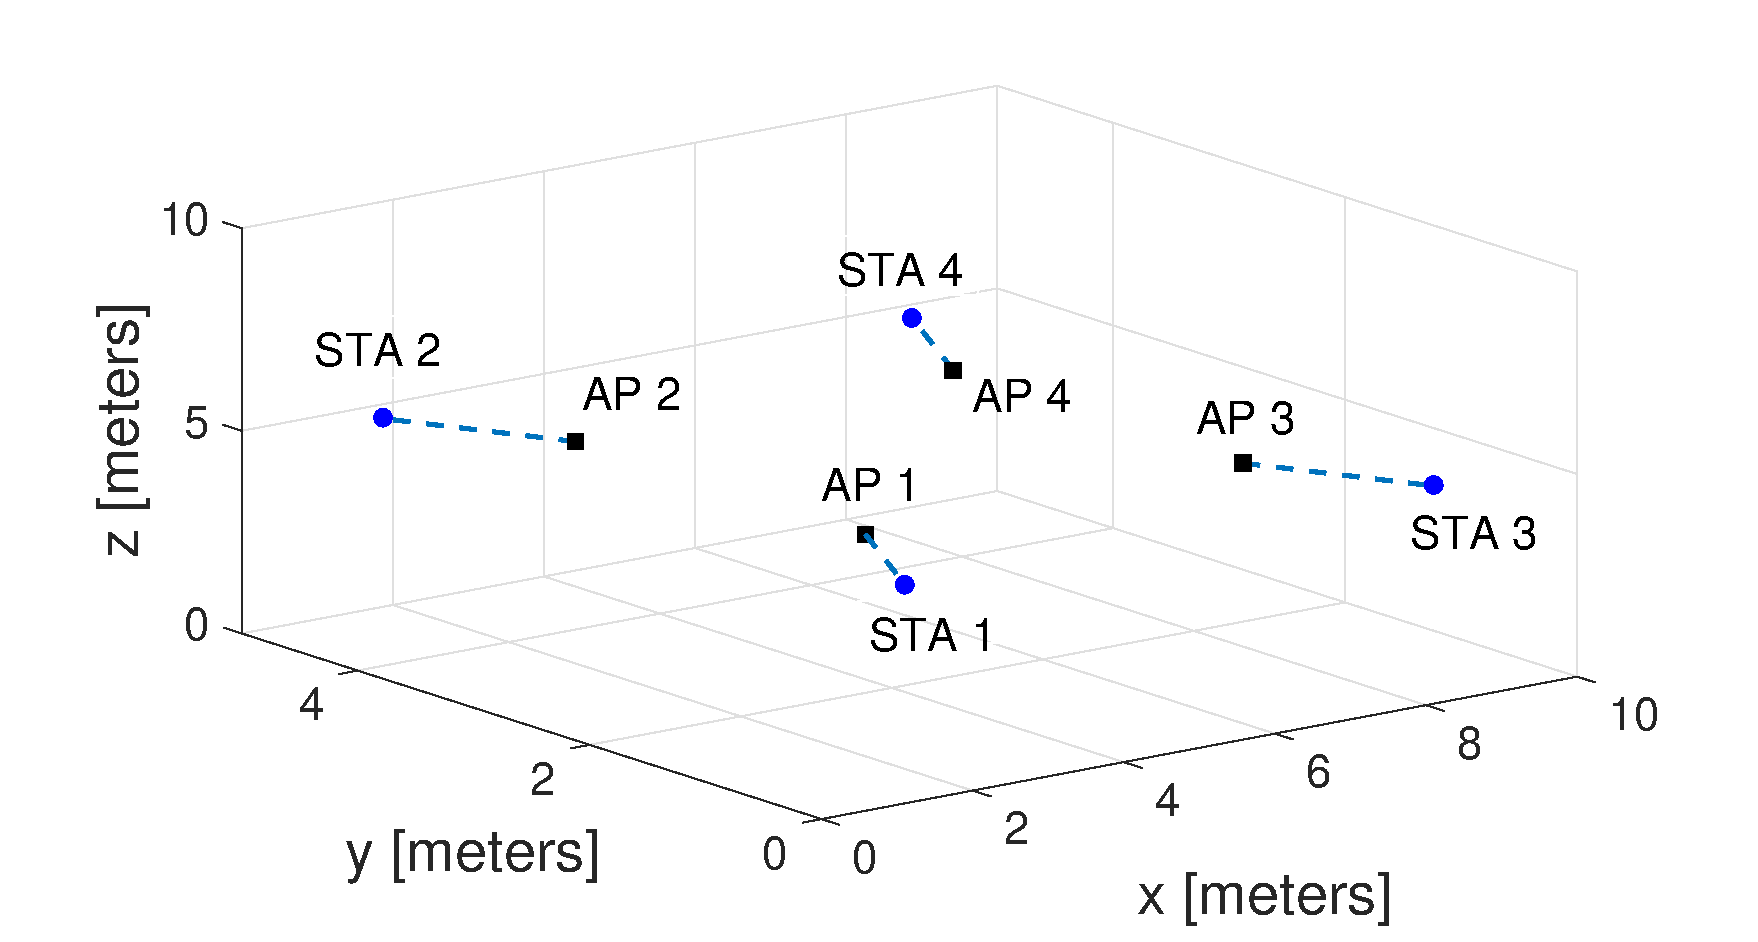
\epsfig{file=images/4_WLANs_scenario.eps, width=8.5cm}
	\caption{Grid scenario containing 4 WNs, each one composed by an AP and a STA.}
	\label{fig:scenario}
\end{figure}

%------------------------
% Optimality study
%------------------------
\subsubsection{Optimal Solution}
\label{section:optimal_solution}	
Before presenting the simulation results of applying a particular action-selection policy, we introduce the optimal solutions that: \emph{i)} maximize the aggregate throughput and \emph{ii)} correspond to proportional fairness\footnote{The proportional fairness solutions satisfy $\underset{a_k \in \mathcal{A}}{\rm max} \sum_{i \in \mathcal{WN}} \log(\Gamma_{i,a_k})$.} for the considered grid scenario, shown in Figure \ref{fig:scenario}.  %Knowing the maximum achievable performance in the presented scenario allows us to provide a meaningful comparison of the introduced policies to be followed by the WNs. 

Let actions range from $a_1$ to $a_8$, and map to \{channel number, transmit power (dBm)\}: $a_1$ = \{1, 5\}, $a_2$ = \{2, 5\}, $a_3$ = \{1, 10\}, $a_4$ = \{2, 10\}, $a_5$ = \{1, 15\}, $a_6$ = \{2, 15\}, $a_7$ = \{1, 20\} and $a_8$ = \{2, 20\}. According to our model, the joint configuration of the 4 WNs that grants the maximum aggregate throughput is any combination of actions \{$a_1$, $a_7$, $a_8$\}, subject to the condition of two close WNs using $a_1$. Despite the scenario is symmetric, the distance between APs is not the same in all the cases. For instance, $d_{\text{AP}_1,\text{AP}_2} > d_{\text{AP}_1,\text{AP}_4}$. It is important to emphasize that the proposed scenario does not consider asymmetries between WNs, so that dominance relationships are not present. In case of suffering from such asymmetries, the performance of a given WN would depend on the configuration of its neighboring networks but it won't be able to affect their behavior. For instance, a WN in the middle of two others may suffer from flow starvation if the WNs in the extremes do not sense each other. In such a situation, the WN in the middle is not able to fairly compete for channel resources due to the asymmetric situation it suffers.
	
In our symmetric scenario, the optimal aggregate throughput is 1124 Mbps, and is only achieved when two consecutive WNs sacrifice themselves by choosing a lower transmit power (action $a_1$). Moreover, to maximize the proportional fairness, the optimal joint configuration changes to any combination using the maximum transmit power (i.e., $a_7$ and $a_8$), so that frequency reuse is maximized; WNs using the same channel must be as much separated as possible. Such a configuration leads to an aggregate throughput of 891 Mbps, which is quite lower than in the former case, but allows experiencing a fairer configuration. Note that all WNs obtain the same throughput in this case as frequency reuse is achieved (closer WNs choose different channels), but power is kept equal for each WN and despite experiencing higher interference, none of the WNs sacrifice themselves. The aim of the following performance evaluation is to gain insight into whether a collaborative result, close to this equal division of resources given by the proportional fair action selection, is likely to be learned by the algorithms and if so, under which conditions.

%------------------------
% Study of MAB (e-greedy)
%------------------------
\subsubsection{Performance of the $\varepsilon$-greedy policy}
\label{section:egreedy_study}	
We first evaluate the performance of the $\varepsilon$-greedy policy when applied to the WNs problem, which allows us to study the purest form of the exploitation-exploration trade-off. First, we show the impact of modifying the initial exploration coefficient, $\varepsilon_0$ (recall that we have considered $\varepsilon_t = \varepsilon_0 / \sqrt{t}$), on the average throughput experienced by the overlapping WNs. Figure \ref{fig:egreedy_tuning_parameters} shows the aggregate throughput obtained in the grid scenario when applying $\varepsilon$-greedy during 10,000 iterations, and for each $\varepsilon_0$ value between 0 and 1 in 0.1 steps. The average and standard deviation of the throughput from 100 simulation runs are shown, which are compared with the optimal throughput presented in Section \ref{section:optimal_solution}.
\begin{figure}[t!]
	\centering							
	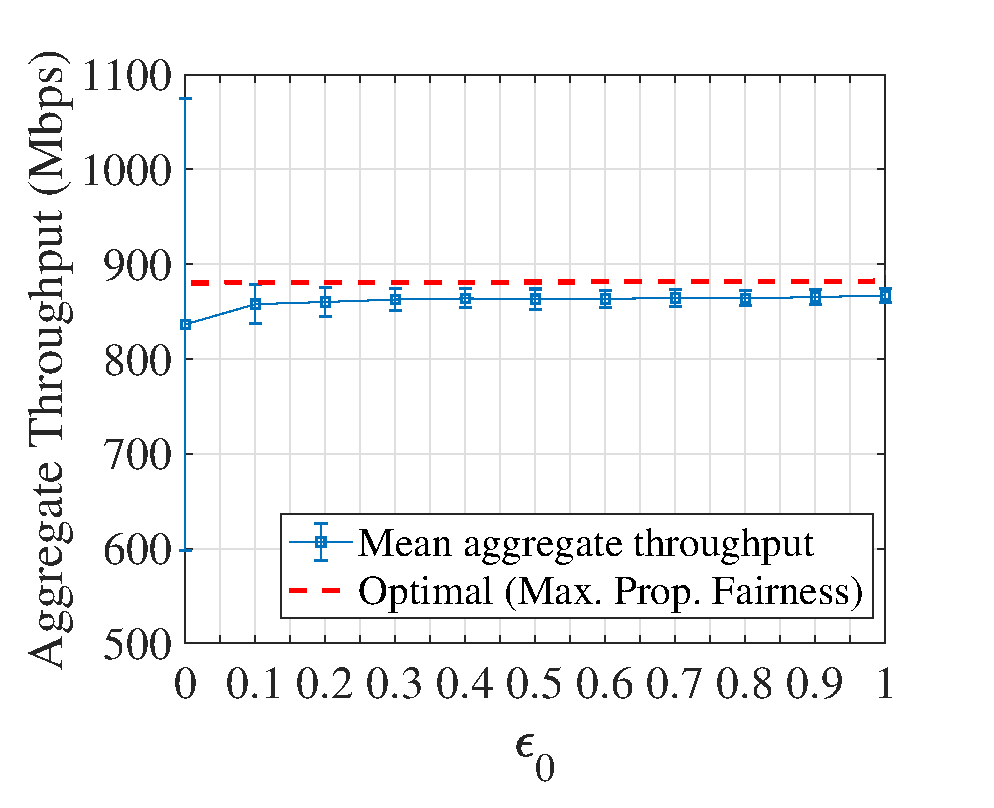
\epsfig{file=images/egreedy_tuning_parameters_zoom.eps, width=6.5cm}
	\caption{Average aggregate throughput and standard deviation obtained for each $\varepsilon_0$ value in $\varepsilon$-greedy. Results are from 100 simulations lasting 10,000 iterations each. The proportional fair solution is also shown (red dashed line).}
	\label{fig:egreedy_tuning_parameters}
\end{figure}		
As shown in the figure, the aggregate throughput obtained in average is quite similar for all the provided values of $\varepsilon_0$, except for the complete random case where no exploration is done ($\varepsilon_0 = 0$). The lower the $\varepsilon_0$ parameter, the less exploration is performed. Consequently, for low $\varepsilon_0$, the average throughput is highly dependent on how good/bad were the actions taken at the beginning of the learning process, which results in a higher standard deviation as $\varepsilon_0$ goes to 0.

Now, in order to provide a deeper analysis on the WNs behavior when implementing the $\varepsilon$-greedy policy, we focus on the actions probability and the temporal evolution of throughput derived from a single simulation run. To this aim, we use $\varepsilon_0 = \{0.1, 0.5, 1\}$, which correspond to three representative cases (low exploration, middle degree of exploration and intensive exploration). Figure \ref{fig:eg_actions_distr} shows the action probability distribution at each WN at the end of the 10,000 iteration-long simulation, and for each of the selected $\varepsilon_0$ values. 

\begin{figure*}
	\centering
	\begin{tabular}{@{}c@{}}
		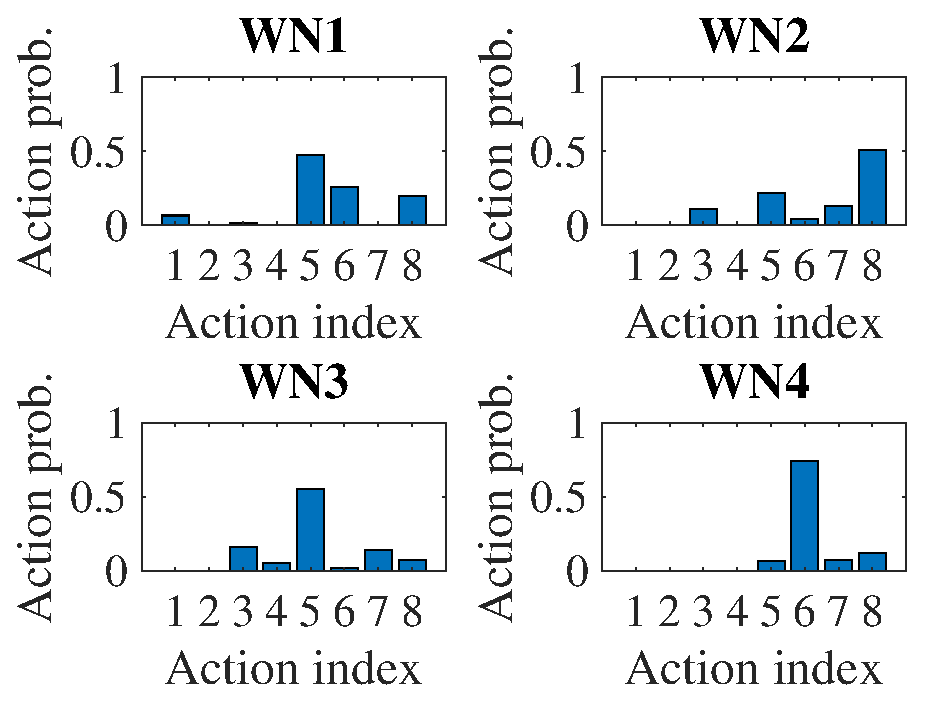
\includegraphics[width=.3\textwidth]{images/NEW_actions_probability_e-greedy_e01} \\[\abovecaptionskip]
		\small (a) $\varepsilon_0$ = 0.1
		\label{fig:eg_e01_actions_distr}
	\end{tabular}	
	\hspace{\floatsep}	
	\begin{tabular}{@{}c@{}}
		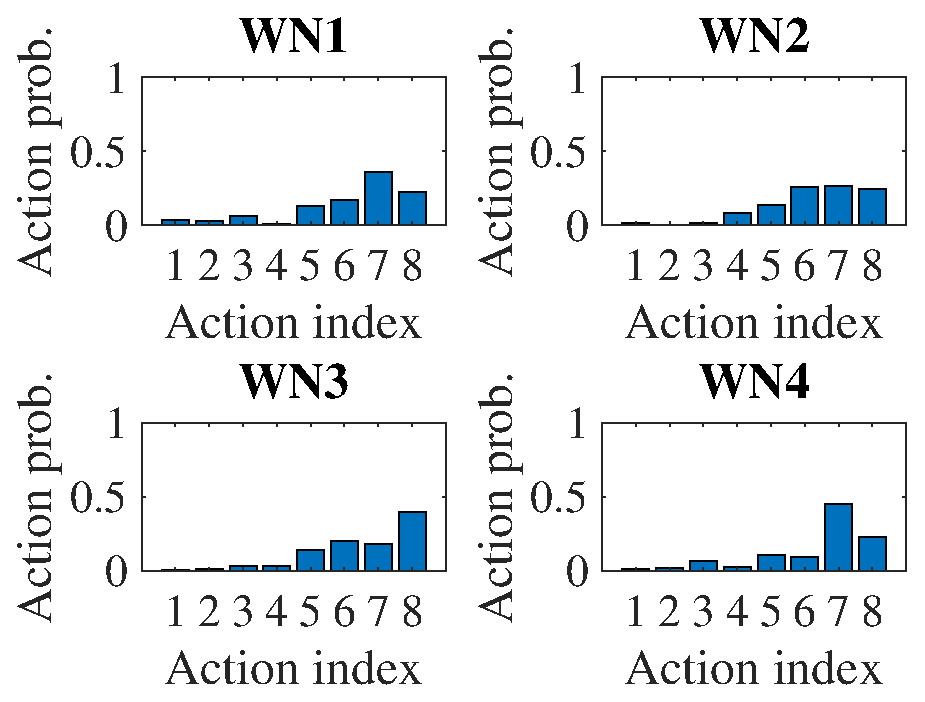
\includegraphics[width=.3\textwidth]{images/NEW_actions_probability_e-greedy_e05} \\[\abovecaptionskip]
		\small (b) $\varepsilon_0$ = 0.5
		\label{fig:eg_e05_actions_distr}
	\end{tabular}
	\hspace{\floatsep}
	\begin{tabular}{@{}c@{}}
		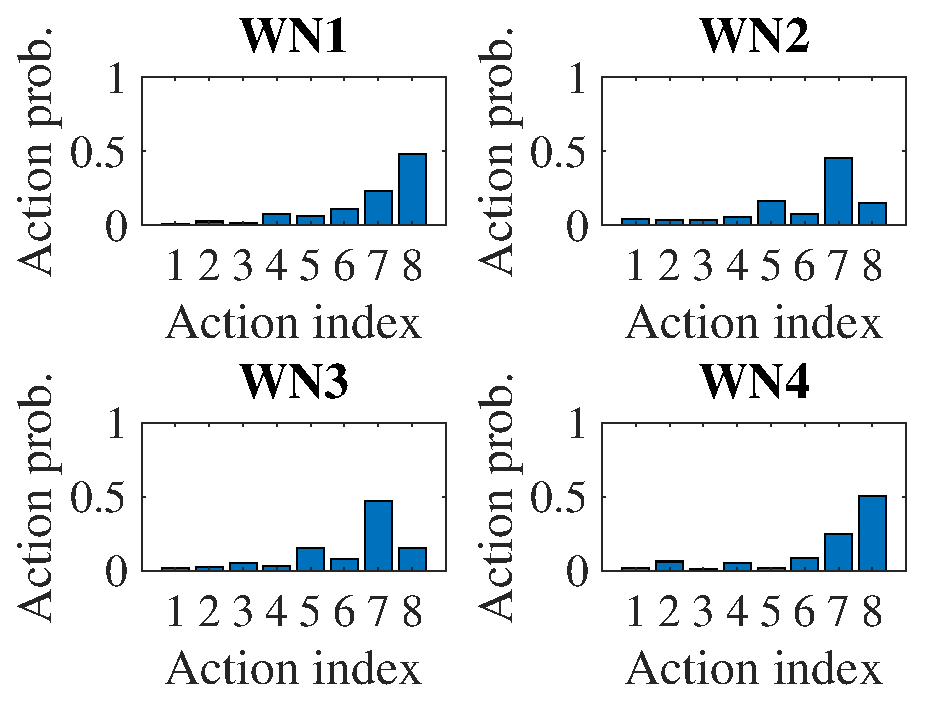
\includegraphics[width=.3\textwidth]{images/NEW_actions_probability_e-greedy_e1} \\[\abovecaptionskip]
		\small (c) $\varepsilon_0$ = 1
		\label{fig:eg_1_actions_distr}
	\end{tabular}
	\caption{Probability of taking a given action in $\varepsilon$-greedy for different $\varepsilon_0$ values after a simulation of 10,000 iterations.}
	\label{fig:eg_actions_distr}
\end{figure*}

We observe in this figure that more aggressive actions (i.e., the ones that use the maximum transmit power) are chosen with a higher rate in all the WNs as $\varepsilon_0$ increases. A higher degree of exploration allows WNs to observe the effects of the actions taken by the others, thus acting in consequence. Accordingly, WNs alternate good/poor performance depending on the actions of the others, which at the same time are also selected intermittently. Despite using a high transmit power allows obtaining a better SNR at the receivers, the generated interference at times becomes counter-productive in terms of individual and aggregate throughput.	

On the other hand, as $\varepsilon_0$ decreases (refer to Figure \ref{fig:eg_actions_distr}(a)), WNs are prone to exploit the same action more frequently, which are the ones that provide the highest known performance. This low degree of exploration results also in a smaller usage of suboptimal actions. 

Figure \ref{fig:eg_agg_tpt}  shows the aggregate throughput evolution, which suffers from higher temporal variability as $\varepsilon_0$ increases. The same observation can be done from the individual throughput evolution (shown in Figure \ref{fig:eg_ind_tpt}), which in addition shows larger differences between the individual patterns for lower $\varepsilon_0$ values. These differences correspond to unfair performance resulting from a low degree of exploration.
% e-greedy: aggregate throughput
\begin{figure*}
	\centering
	\begin{tabular}{@{}c@{}}
		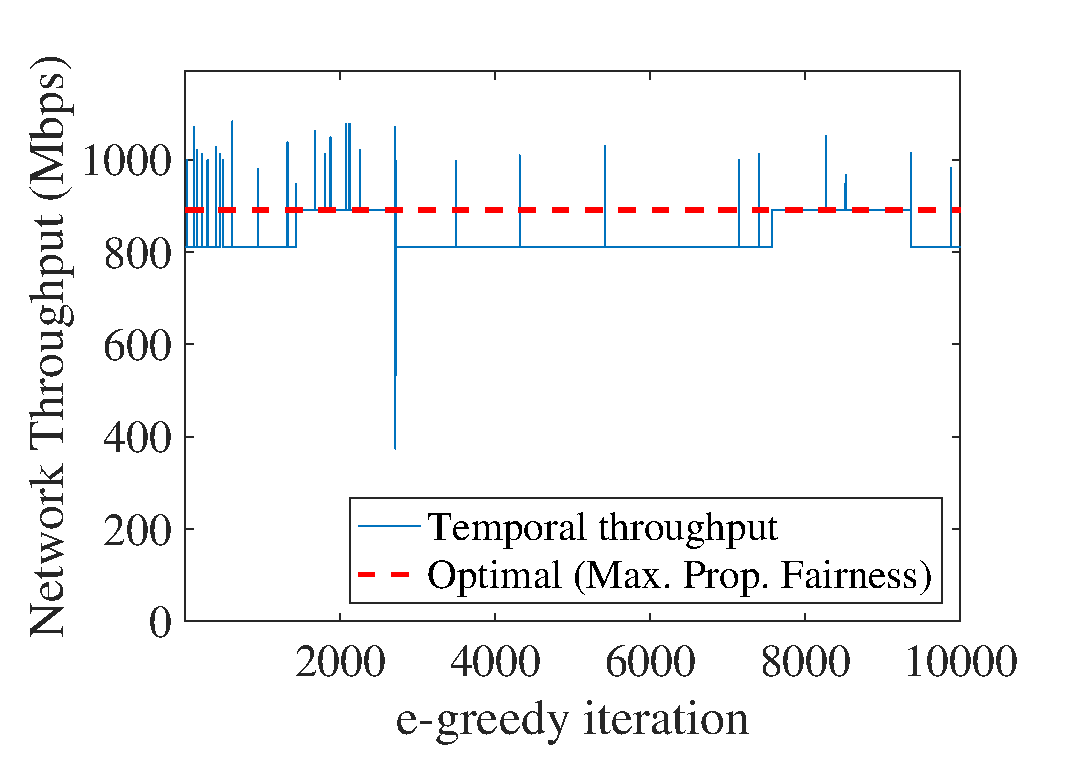
\includegraphics[width=.3\textwidth]{images/NEW_temporal_aggregate_tpt_e-greedy_e01} \\[\abovecaptionskip]
		\small (a) $\varepsilon_0$ = 0.1
		\label{fig:eg_e01_agg_tpt}
	\end{tabular}	
	\hspace{\floatsep}	
	\begin{tabular}{@{}c@{}}
		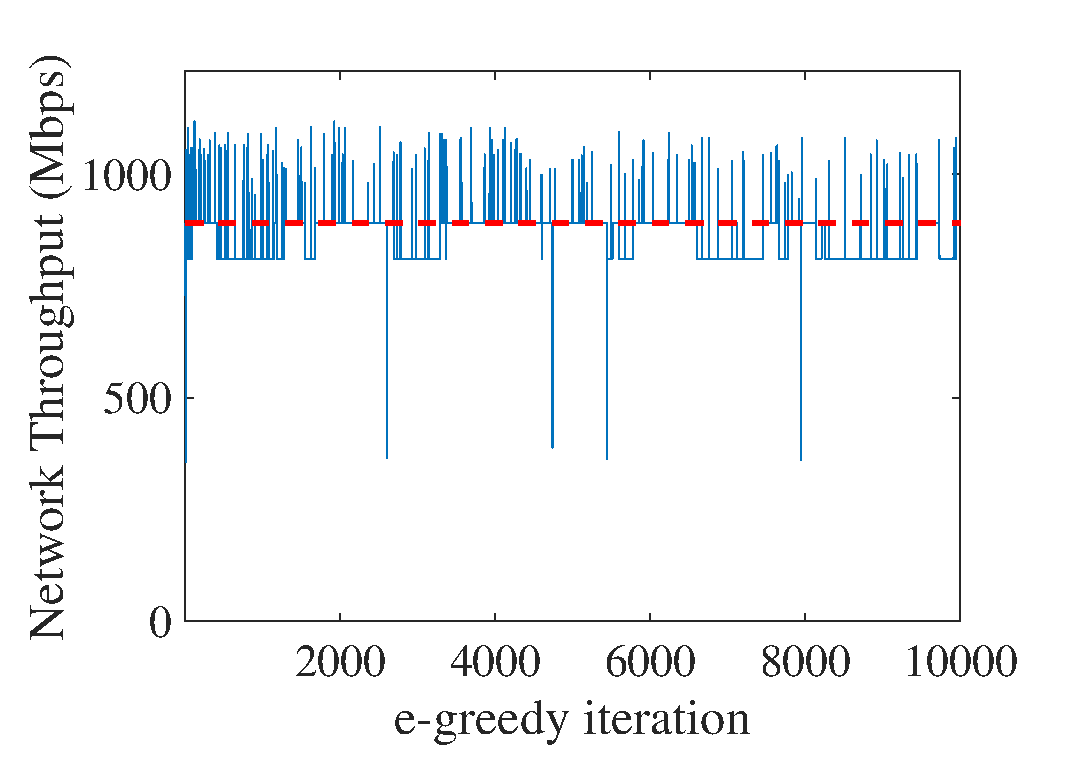
\includegraphics[width=.3\textwidth]{images/NEW_temporal_aggregate_tpt_e-greedy_e05} \\[\abovecaptionskip]
		\small (b) $\varepsilon_0$ = 0.5
		\label{fig:eg_e05_agg_tpt}
	\end{tabular}
	\hspace{\floatsep}
	\begin{tabular}{@{}c@{}}
		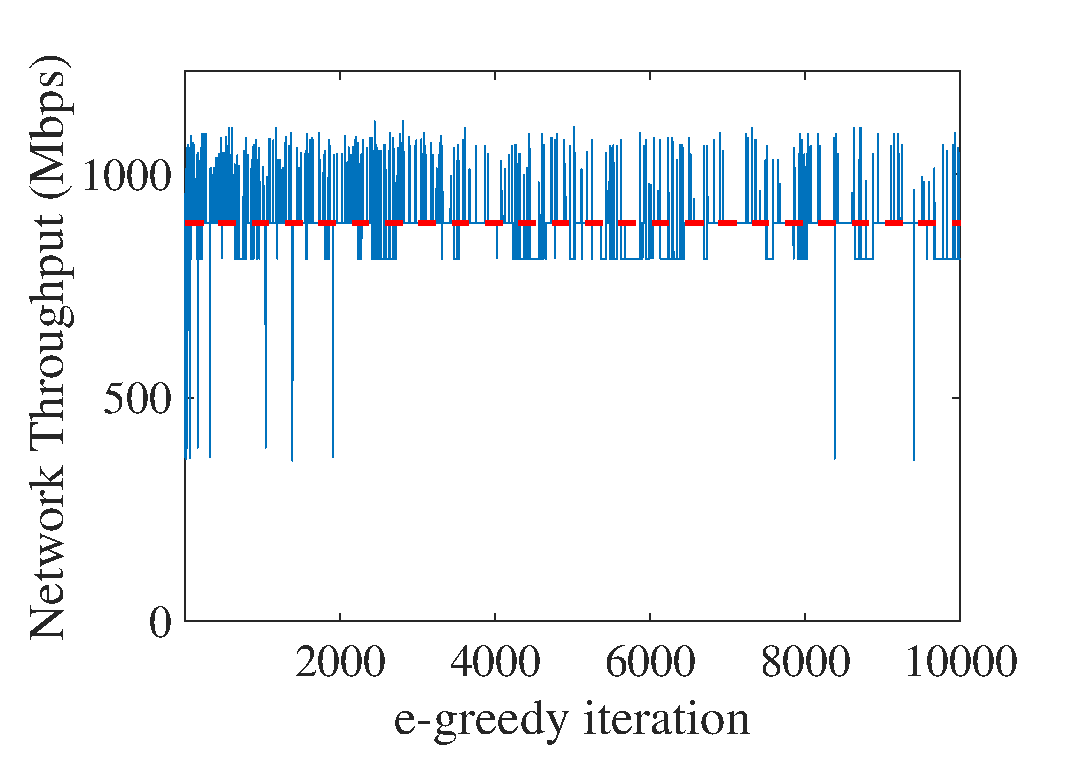
\includegraphics[width=.3\textwidth]{images/NEW_temporal_aggregate_tpt_e-greedy_e1} \\[\abovecaptionskip]
		\small (c) $\varepsilon_0$ = 1
		\label{fig:eg_e1_agg_tpt}
	\end{tabular}
	\caption{Aggregate throughput evolution for a single $\varepsilon$-greedy 10,000-iterations simulation and for different $\varepsilon_0$ values. The proportional fair result is also shown (red dashed line).}
	\label{fig:eg_agg_tpt}
\end{figure*}

% e-greedy: individual throughput
\begin{figure*}
	\centering
	\begin{tabular}{@{}c@{}}
		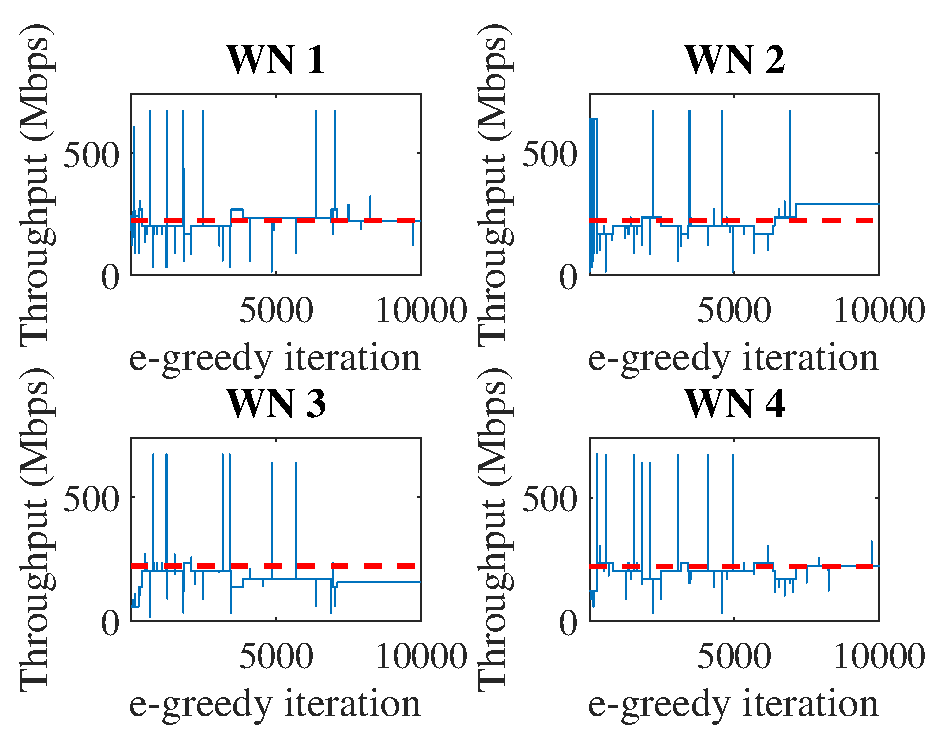
\includegraphics[width=.3\textwidth]{images/NEW_temporal_individual_tpt_e-greedy_e01} \\[\abovecaptionskip]
		\small (a) $\varepsilon_0$ = 0.1
		\label{fig:eg_e01_ind_tpt}
	\end{tabular}	
	\hspace{\floatsep}	
	\begin{tabular}{@{}c@{}}
		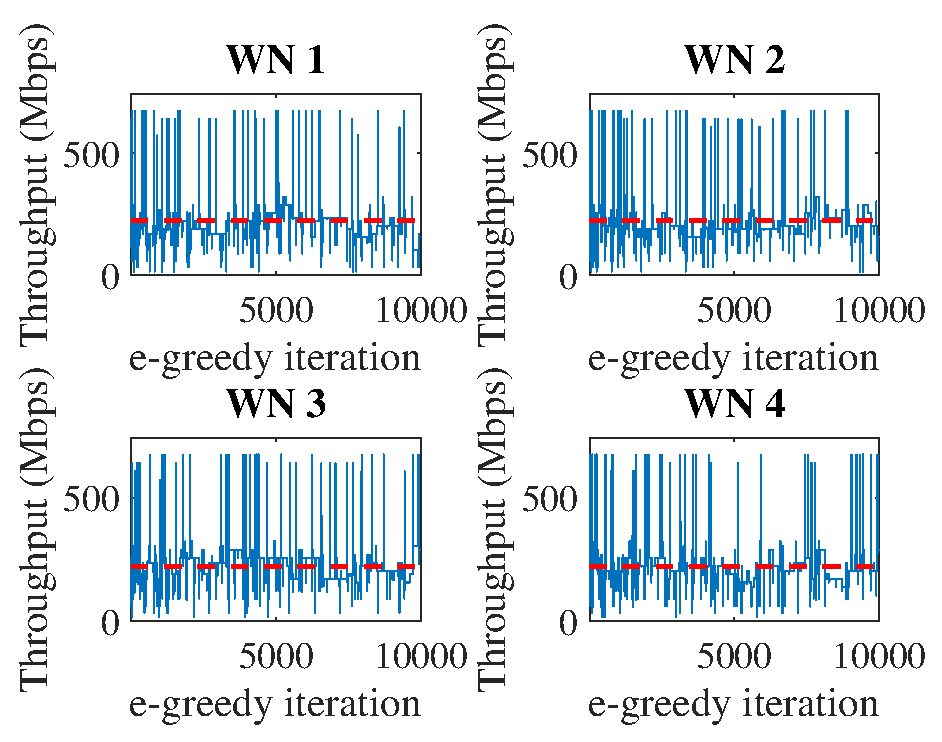
\includegraphics[width=.3\textwidth]{images/NEW_temporal_individual_tpt_e-greedy_e05} \\[\abovecaptionskip]
		\small (b) $\varepsilon_0$ = 0.5
		\label{fig:eg_e05_ind_tpt}
	\end{tabular}
	\hspace{\floatsep}
	\begin{tabular}{@{}c@{}}
		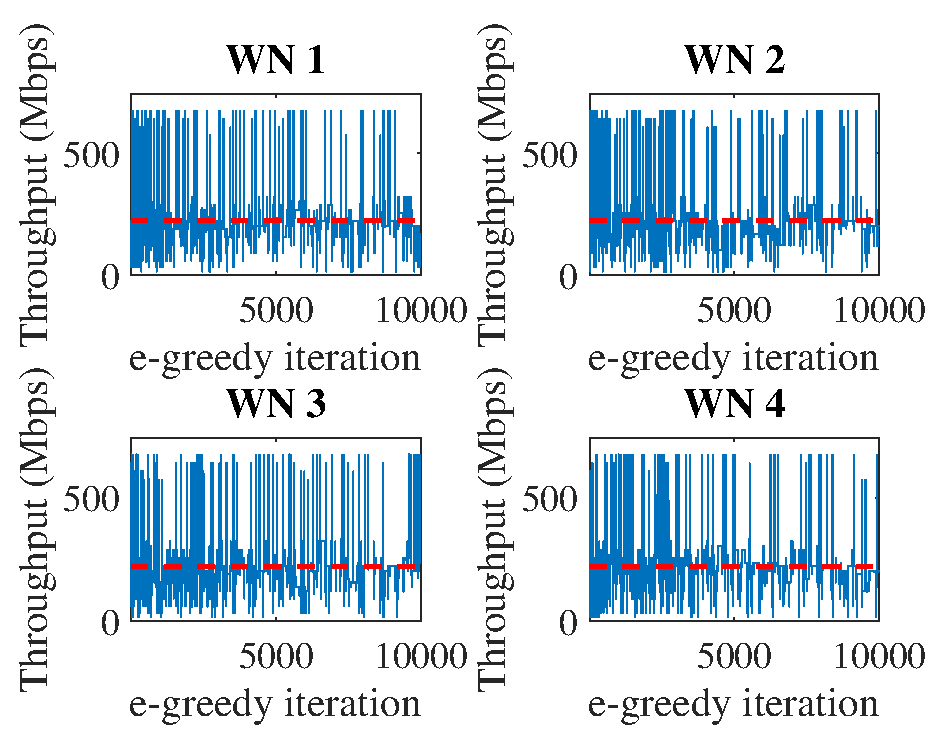
\includegraphics[width=.3\textwidth]{images/NEW_temporal_individual_tpt_e-greedy_e1} \\[\abovecaptionskip]
		\small (c) $\varepsilon_0$ = 1
		\label{fig:eg_e1_ind_tpt}
	\end{tabular}
	\caption{Individual throughput evolution for a single $\varepsilon$-greedy 10,000-iterations simulation and for different $\varepsilon_0$ values. The proportional fair result is also shown (red dashed line).}
	\label{fig:eg_ind_tpt}
\end{figure*}

To gain further insight into fairness, we depict in Figure \ref{fig:eg_avg_tpt} the average  and standard deviation of the throughput at each WN. We have now concentrated in the last 5,000 iterations of the simulation, disregarding the instability provoked during the transitory regime, so that we get a better picture of the long-term behavior. We see that as $\varepsilon_0$ increases, the experienced fairness becomes higher due to the temporal fluctuation that occurs as a consequence of performing more exploratory actions. Moreover, we also observe that the standard deviation of the throughput is similar at each WN.  

% e-greedy: average throughput
\begin{figure*}
	\centering
	\begin{tabular}{@{}c@{}}
		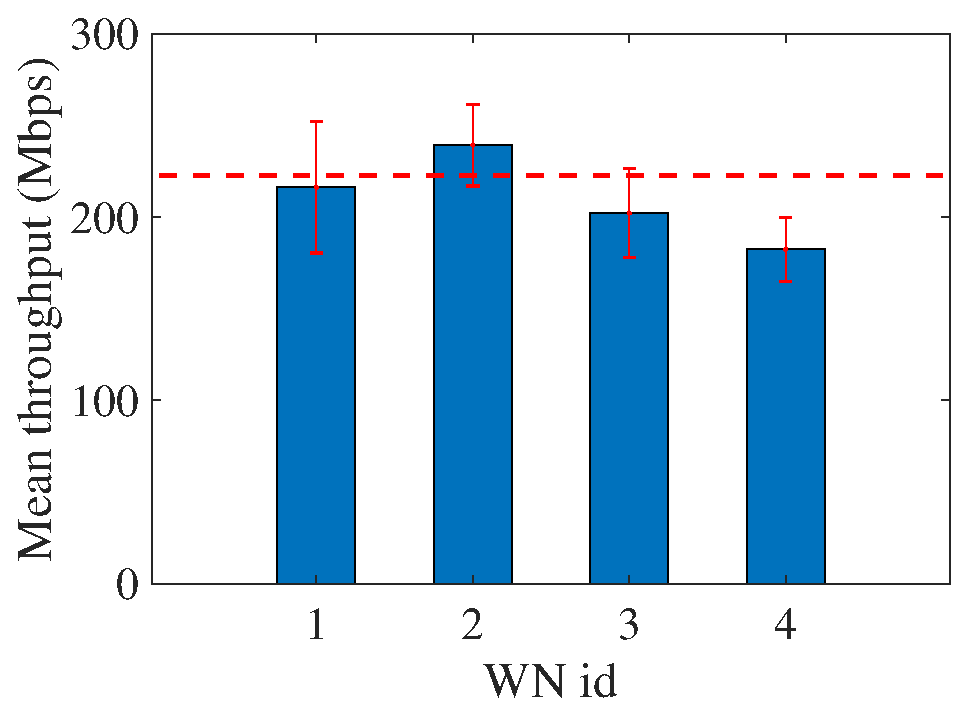
\includegraphics[width=.3\textwidth]{images/NEW_mean_tpt_e-greedy_e01} \\[\abovecaptionskip]
		\small (a) $\varepsilon_0$ = 0.1
		\label{fig:eg_e01_avg_tpt}
	\end{tabular}	
	\hspace{\floatsep}	
	\begin{tabular}{@{}c@{}}
		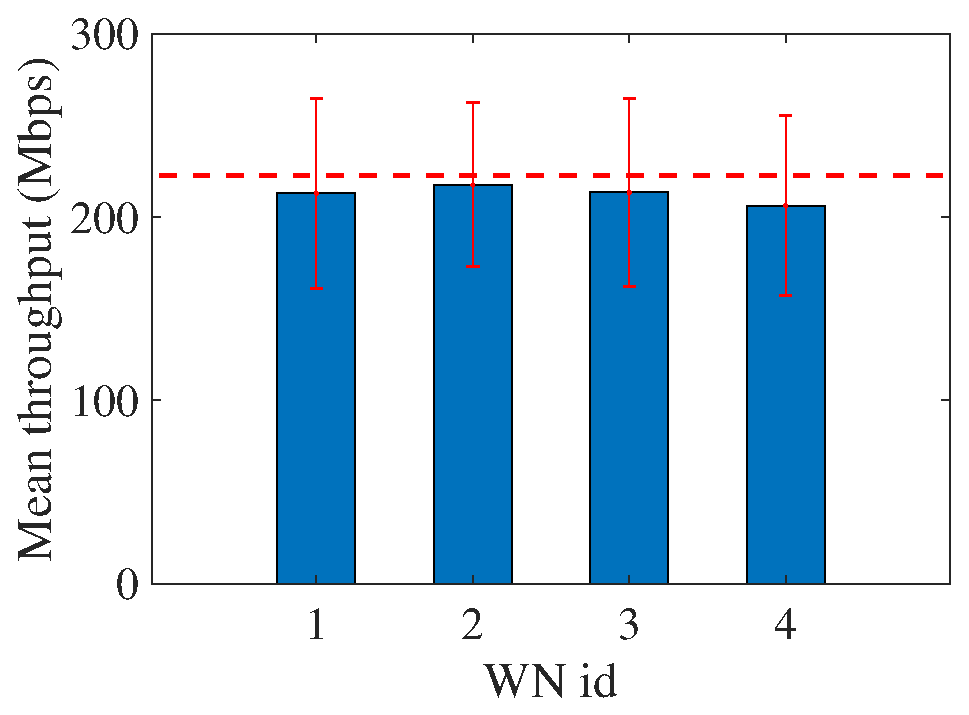
\includegraphics[width=.3\textwidth]{images/NEW_mean_tpt_e-greedy_e05} \\[\abovecaptionskip]
		\small (b) $\varepsilon_0$ = 0.5
		\label{fig:eg_e05_avg_tpt}
	\end{tabular}
	\hspace{\floatsep}
	\begin{tabular}{@{}c@{}}
		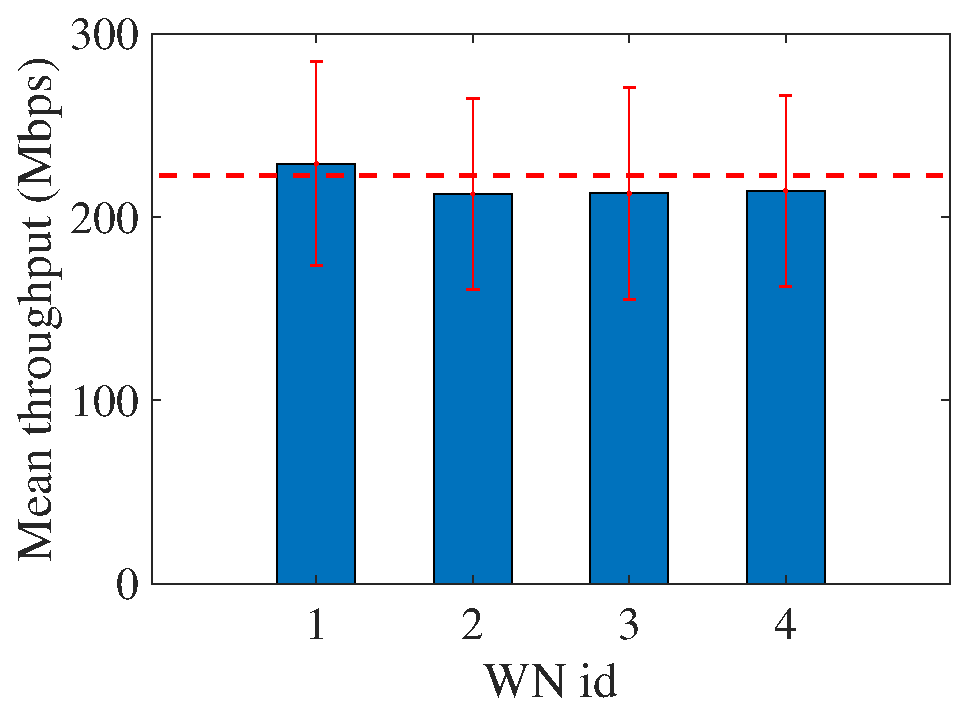
\includegraphics[width=.3\textwidth]{images/NEW_mean_tpt_e-greedy_e1} \\[\abovecaptionskip]
		\small (c) $\varepsilon_0$ = 1
		\label{fig:eg_e1_avg_tpt}
	\end{tabular}
	\caption{Average throughput and standard deviation experienced per WN in the last 5,000 iterations of a single $\varepsilon$-greedy 10,000-iterations simulation run for different $\varepsilon_0$ values. The proportional fair result is also shown (red dashed line).}
	\label{fig:eg_avg_tpt}
\end{figure*}

To sum up, we have seen that tuning $\varepsilon_0$ clearly entails a trade-off between the fairness and the temporal variation of throughput. Choosing a low $\varepsilon_0$ value grants low variability, but WNs are prone to fall into local maximums, as the experienced performance is just a consequence of the randomness in taking particular actions. This also generates a fairness problem, since the unlucky WNs end up experiencing lower performance, as well as they are not able to discover the best throughput actions. On the other side, choosing a high $\varepsilon_0$ value results in higher throughput and better long-term fairness but at the expense of intermittent good/poor performance.

%------------------------
% Study of MAB (EXP3)
%------------------------
\subsubsection{Performance of the EXP3 policy}
\label{section:exp3_study}
We now evaluate the trade-off between fairness and temporal throughput variability in the EXP3 policy, which includes the learning rate $\eta$, a parameter that controls how fast old beliefs are replaced by newer ones. In EXP3 we also find the $\gamma$ parameter, which regulates explicit exploration by tuning the importance of weights in the action-selection procedure. Setting $\gamma = 1$ results in completely neglecting weights (actions have the same probability to be chosen). On the other side, setting $\gamma = 0$, the effect of weights are  at its highest. Thus, in order to see clearly the effects of the EXP3 weights, which directly depend on $\eta$, we fix $\gamma$ to 0.

As we did before for $\varepsilon$-greedy, we start analyzing the impact of modifying the input parameters of EXP3 on the average aggregate throughput (Figure \ref{fig:exp3_tuning_parameters}). We vary the initial learning rate, $\eta_0$, between 0 and 1 in 0.1 steps. As it can be observed, setting $\eta_0$ to 0 results in the lowest average throughput, and a low variability is obtained. In this case, action weights are never updated and the arms are randomly chosen with the same probability. As $\eta_0$ increases, the proportional fair solution is approximated at the expense of a higher variability between experiments, since less exploration is performed when $\eta_0$ increases. Note, as well, that the maximum average network throughput is reached for $\eta_0 = 0.6$ in this particular scenario.

\begin{figure}[t!]
	\centering											
	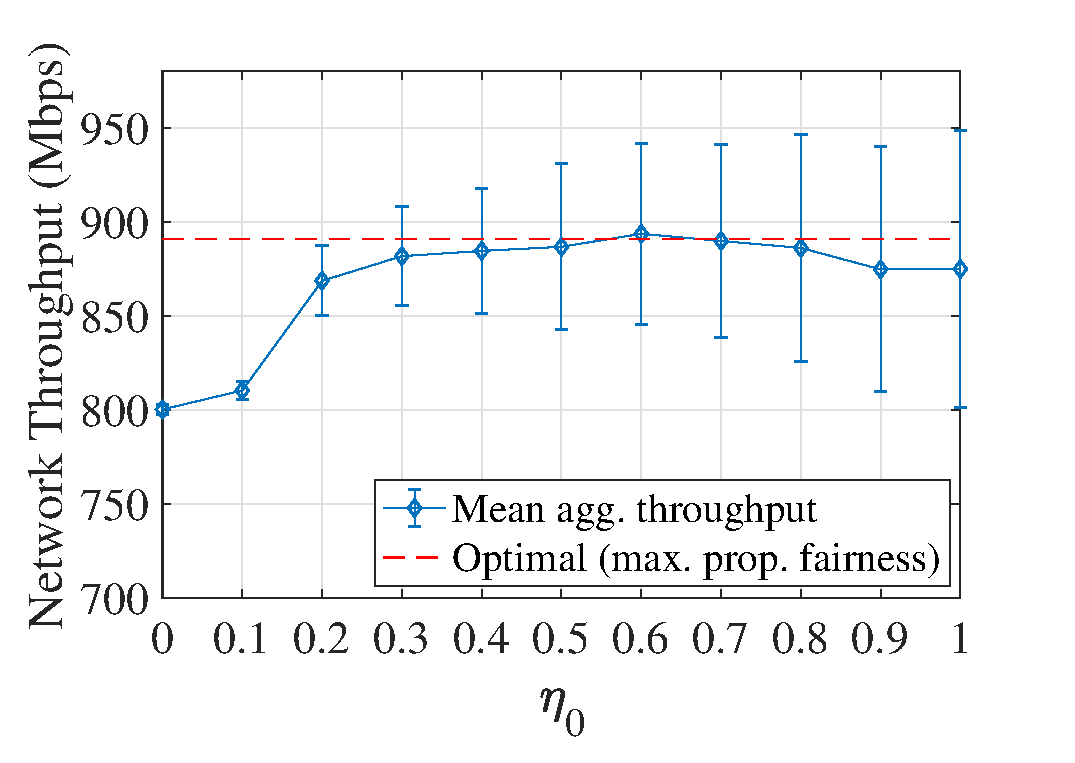
\epsfig{file=images/exp3_tuning_parameters_zoom.eps, width=6.5cm}
	\caption{Average aggregate throughput and standard deviation obtained for each $\eta_0$ value in MAB (EXP3). The aggregate throughput of the proportional fair solution is also shown (red dashed line). Results are from 100 simulations lasting 10,000 iterations each.}
	\label{fig:exp3_tuning_parameters}
\end{figure}	

Now, for a single 10,000-iteration simulation, we set $\eta_0 = \{0.1, 0.5, 1\}$ to closely study the implications of modifying the initial learning rate. Figure \ref{fig:exp3_actions_distr} compares the resulting actions probability for these low, medium and high $\eta_0$ values.
% EXP3: action probabilities
\begin{figure*}
	\centering
	\begin{tabular}{@{}c@{}}
		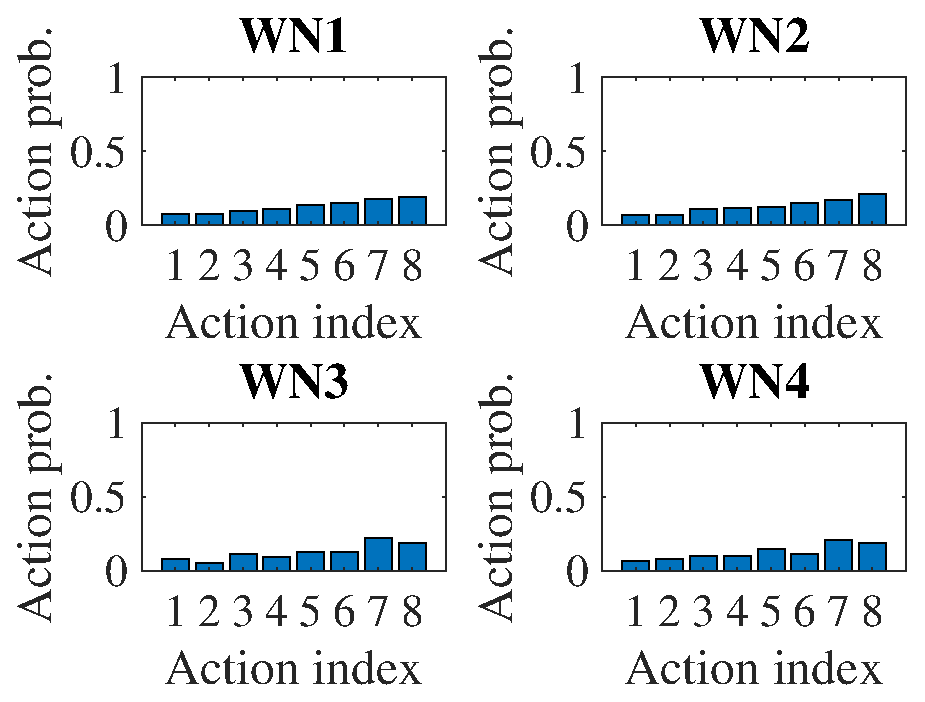
\includegraphics[width=.3\textwidth]{images/NEW_actions_probability_EXP3_eta01} \\[\abovecaptionskip]
		\small (a) $\eta_0 = 0.1$
		\label{fig:exp3_eta01_actions_distr}
	\end{tabular}	
	\hspace{\floatsep}	
	\begin{tabular}{@{}c@{}}
		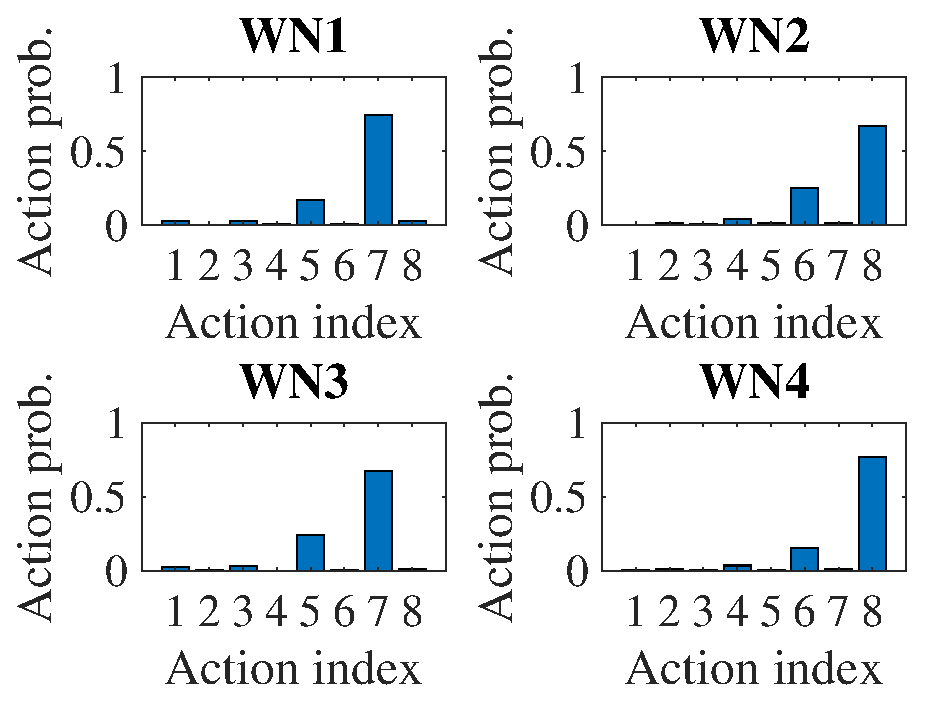
\includegraphics[width=.3\textwidth]{images/NEW_actions_probability_EXP3_eta05} \\[\abovecaptionskip]
		\small (b) $\eta_0 = 0.5$
		\label{fig:exp3_eta05_actions_distr}
	\end{tabular}
	\hspace{\floatsep}
	\begin{tabular}{@{}c@{}}
		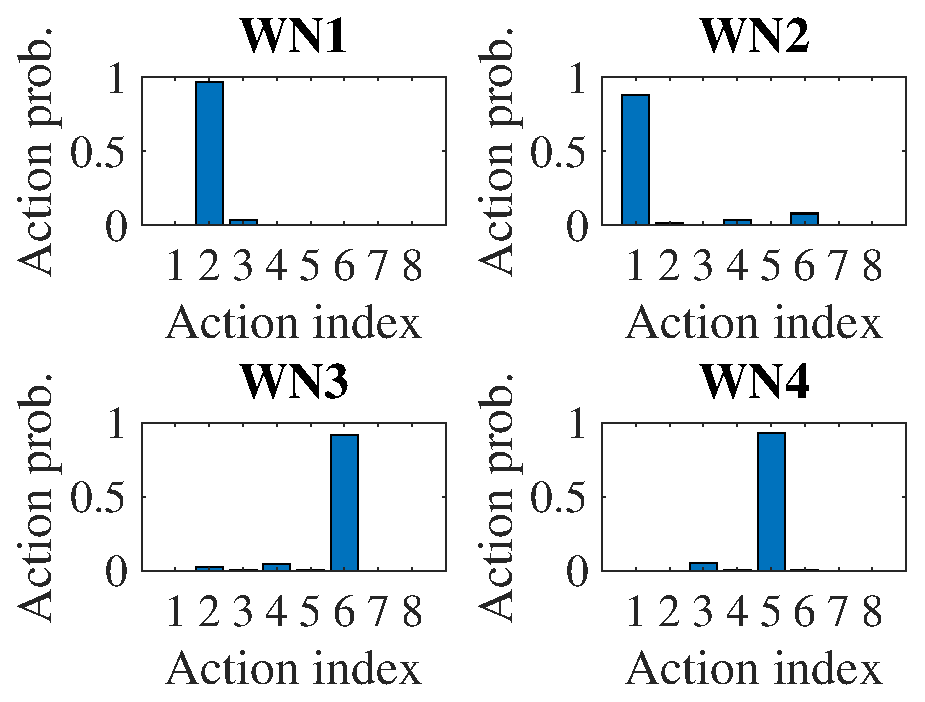
\includegraphics[width=.3\textwidth]{images/NEW_actions_probability_EXP3_eta1} \\[\abovecaptionskip]
		\small (c) $\eta_0 = 1$
		\label{fig:exp3_eta1_actions_distr}
	\end{tabular}
	\caption{Probability of taking a given action in EXP3 for different $\eta_0$ values after a simulation of 10,000 iterations.}
	\label{fig:exp3_actions_distr}
\end{figure*}

We see that actions are tried with similar probability for $\eta_0 = 0.1$, since the usage of a low learning rate entails a high similarity between weights. This situation is significantly improved for $\eta_0 = 0.5$, in which few actions are selected most of the times. The increased learning rate allows to rapidly capture the effects of the others' actions, since more exploration is carried out. As a consequence, actions using the highest transmit power are clearly preferred to overcome the adversarial setting. Note, as well, that optimal channel allocation is learned by WNs despite competing with each other. Finally, for $\eta_0 = 1$, a single action is clearly preferred by each WN. However, unfair situations eventually occur due to the lack of exploration. In particular, we observe that $\text{WN}_1$ and $\text{WN}_3$, which share the same channel, use very different power levels in their favorite actions (5 and 15 dBm, respectively). This, of course, generates a fairness imbalance that favors $\text{WN}_3$, which enjoys a higher SINR. As mentioned, this behavior occurs eventually, since the variability in the output can be understood as a consequence of a fast convergence achieved during the transitory learning phase. So, results from different simulations will significantly vary.

Figure \ref{fig:exp3_agg_tpt} shows the temporal aggregate throughput, which suffers from a higher variability when $\eta$ is lower. Regarding individual performance, the same behavior can be observed in the temporal throughput evolution (Figure \ref{fig:exp3_ind_tpt}). In this case, setting $\eta_0 = 1$ implies trusting best-performing actions for larger periods, i.e., higher weights are assigned even if actions are suboptimal. Therefore, as $\eta_0$ decreases, the temporal variability increases because the action-selection process becomes uniformly random. However, this variability does not entail that the proportional fair solution is approached. Thus, $\eta_0$ must be carefully set in order to provide a low temporal variability, at the same time that enough exploration is carried out for reaching the optimal fairness solution.

% EXP3: aggregate throughput
\begin{figure*}
	\centering
	\begin{tabular}{@{}c@{}}
		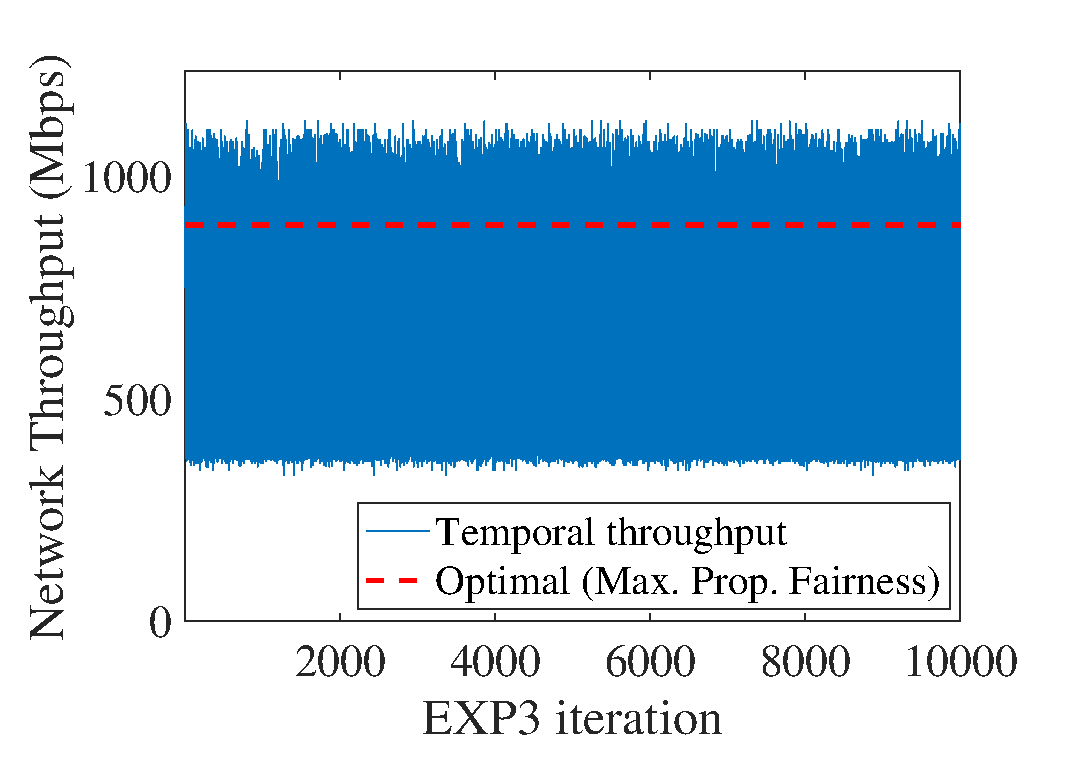
\includegraphics[width=.3\textwidth]{images/NEW_temporal_aggregate_tpt_EXP3_eta01} \\[\abovecaptionskip]
		\small (a) $\eta_0 = 0.1$
		\label{fig:exp3_eta01_agg_tpt}
	\end{tabular}	
	\hspace{\floatsep}	
	\begin{tabular}{@{}c@{}}
		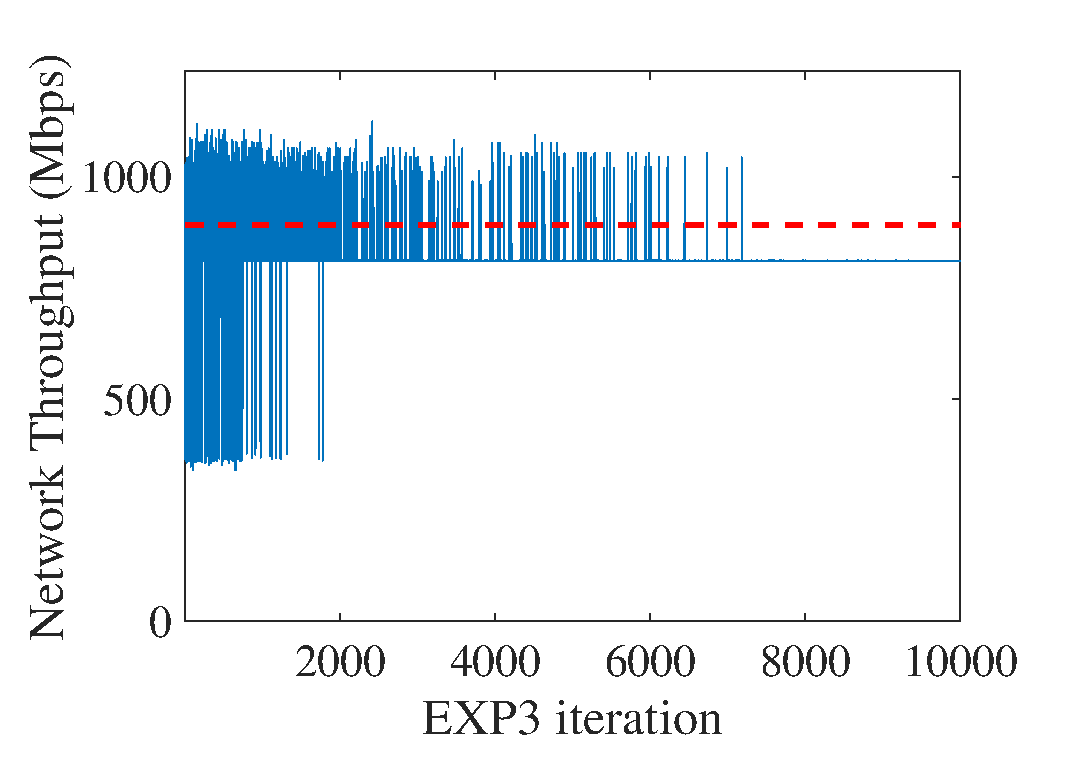
\includegraphics[width=.3\textwidth]{images/NEW_temporal_aggregate_tpt_EXP3_eta05} \\[\abovecaptionskip]
		\small (b) $\eta_0 = 0.5$
		\label{fig:exp3_eta05_agg_tpt}
	\end{tabular}
	\hspace{\floatsep}
	\begin{tabular}{@{}c@{}}
		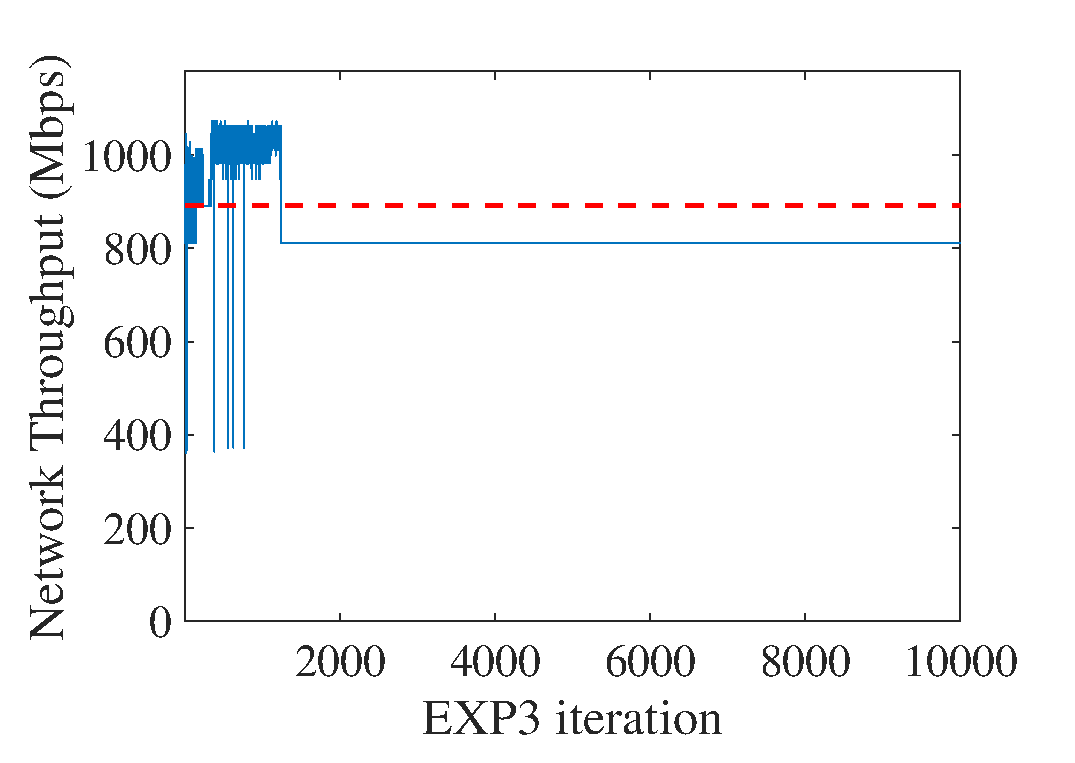
\includegraphics[width=.3\textwidth]{images/NEW_temporal_aggregate_tpt_EXP3_eta1} \\[\abovecaptionskip]
		\small (c) $\eta_0 = 1$
		\label{fig:exp3_eta1_agg_tpt}
	\end{tabular}
	\caption{Aggregate throughput evolution for a single EXP3 10000-iterations simulation and for different $\eta_0$ values. The proportional fair result is also shown (red dashed line).}
	\label{fig:exp3_agg_tpt}
\end{figure*}

% EXP3: individual throughput
\begin{figure*}
	\centering
	\begin{tabular}{@{}c@{}}
		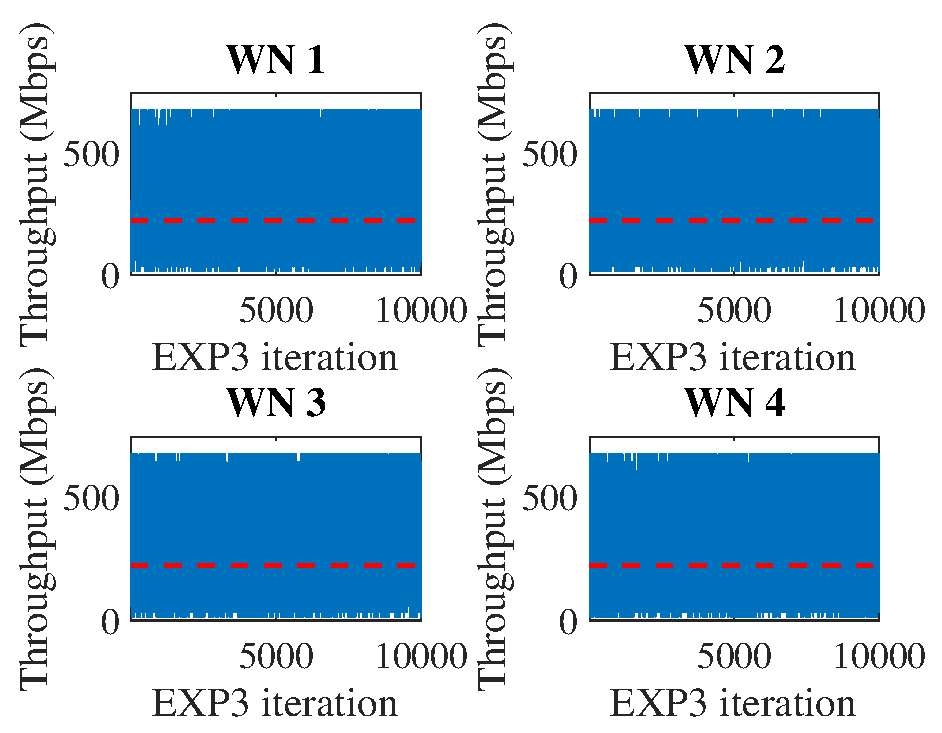
\includegraphics[width=.3\textwidth]{images/NEW_temporal_individual_tpt_EXP3_eta01} \\[\abovecaptionskip]
		\small (a) $\eta_0 = 0.1$
		\label{fig:exp3_eta01_ind_tpt}
	\end{tabular}	
	\hspace{\floatsep}	
	\begin{tabular}{@{}c@{}}
		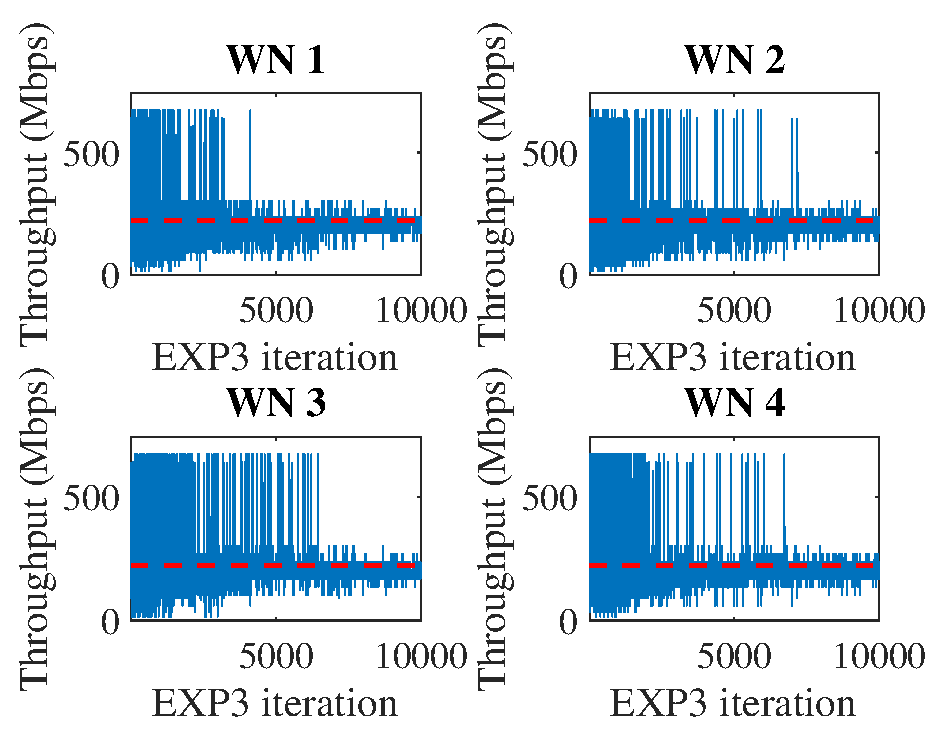
\includegraphics[width=.3\textwidth]{images/NEW_temporal_individual_tpt_EXP3_eta05} \\[\abovecaptionskip]
		\small (b) $\eta_0 = 0.5$
		\label{fig:exp3_eta05_ind_tpt}
	\end{tabular}
	\hspace{\floatsep}
	\begin{tabular}{@{}c@{}}
		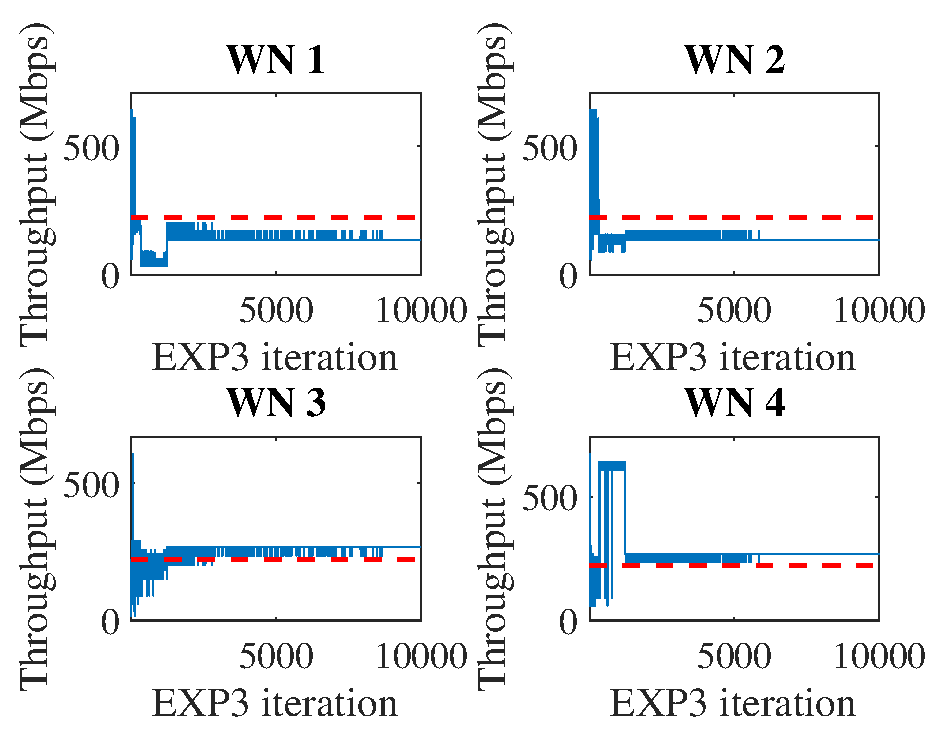
\includegraphics[width=.3\textwidth]{images/NEW_temporal_individual_tpt_EXP3_eta1} \\[\abovecaptionskip]
		\small (c) $\eta_0 = 1$
		\label{fig:exp3_eta1_ind_tpt}
	\end{tabular}
	\caption{Individual throughput evolution for a single EXP3 10000-iterations simulation and for different $\eta_0$ values. The proportional fair result is also shown (red dashed line).}
	\label{fig:exp3_ind_tpt}
\end{figure*}

One can notice a fairness imbalance by observing the individual throughput for $\eta_0 = 1$ in Figure \ref{fig:exp3_ind_tpt}, which is further illustrated in Figure \ref{fig:exp3_avg_tpt} (again, we have considered the last 5,000 iterations to avoid capturing the transitory phase). The average throughput is more evenly distributed for $\eta_0 = 0.1$ and $\eta_0 = 0.5$, but at the expense of the experienced throughput variability seen above. The unfairness suffered for $\eta_0 = 0.1$ can be understood as a lack of exploration that prevents finding a fair resource distribution. Thus, we conclude that a similar trade-off experienced in $\varepsilon$-greedy appears in EXP3 with parameter $\eta_0$. The main difference is that, in this case, a random action-selection process is approximated as $\eta_0$ decreases.
% EXP3: average throughput
\begin{figure*}
	\centering
	\begin{tabular}{@{}c@{}}
		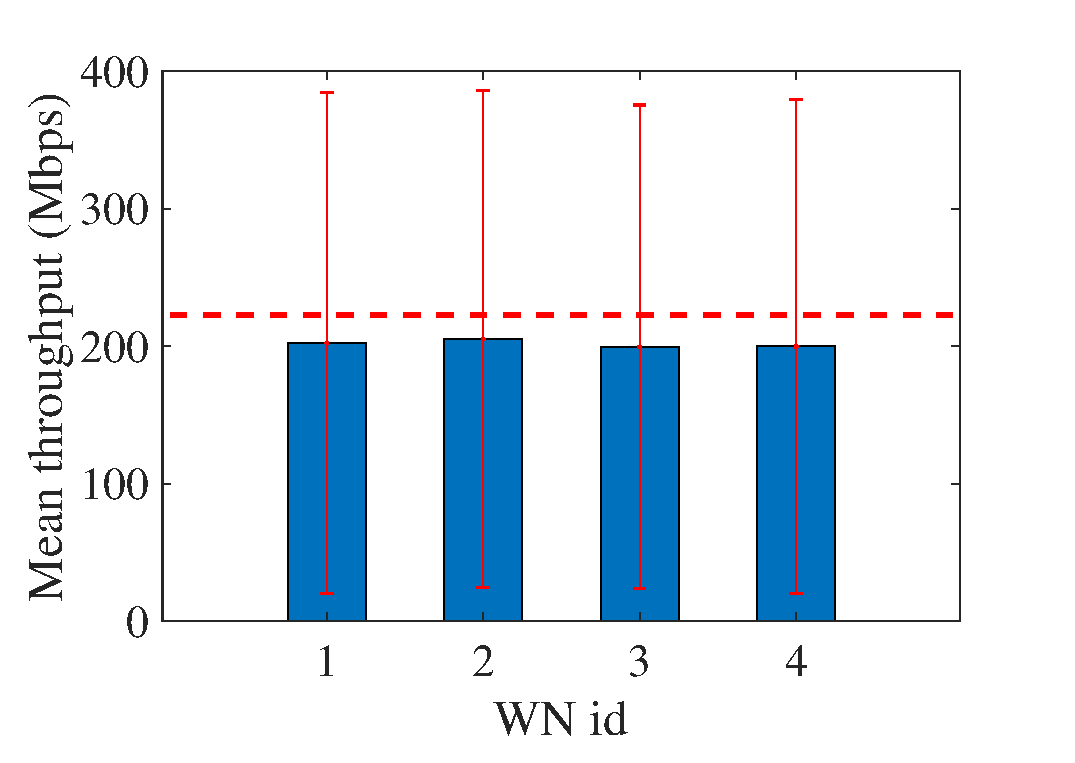
\includegraphics[width=.3\textwidth]{images/NEW_mean_tpt_EXP3_eta01} \\[\abovecaptionskip]
		\small (a) $\eta_0 = 0.1$
		\label{fig:exp3_eta01_avg_tpt}
	\end{tabular}	
	\hspace{\floatsep}	
	\begin{tabular}{@{}c@{}}
		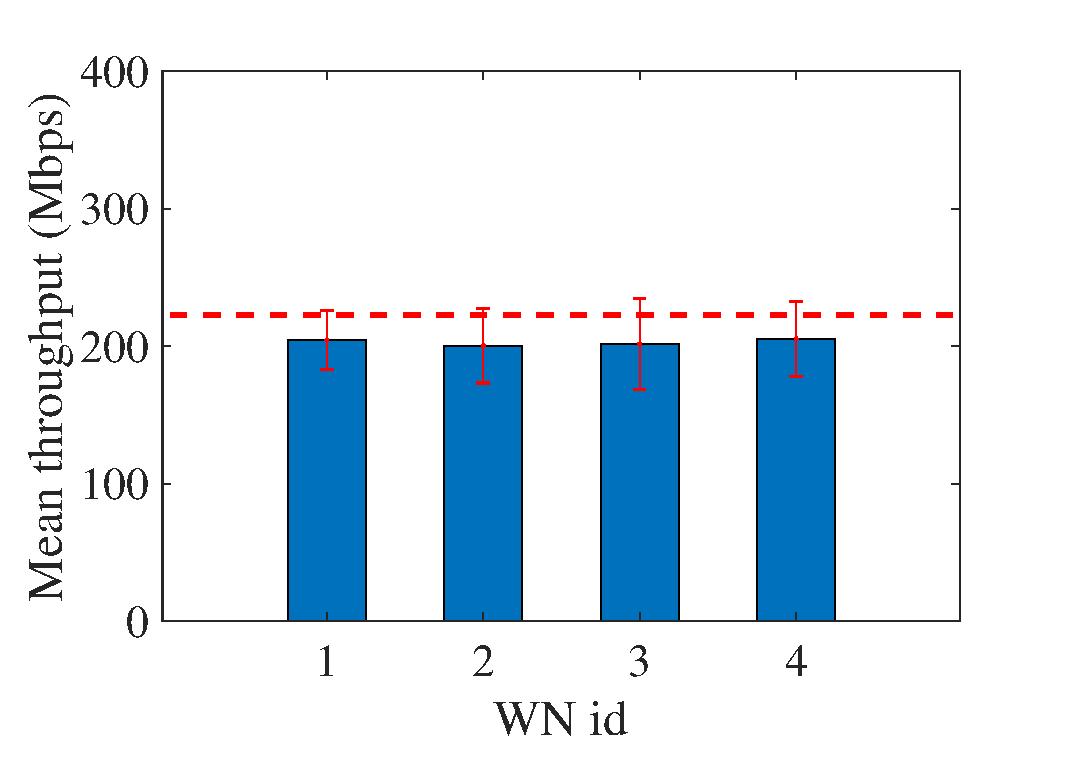
\includegraphics[width=.3\textwidth]{images/NEW_mean_tpt_EXP3_eta05} \\[\abovecaptionskip]
		\small (b) $\eta_0 = 0.5$
		\label{fig:exp3_eta05_avg_tpt}
	\end{tabular}
	\hspace{\floatsep}
	\begin{tabular}{@{}c@{}}
		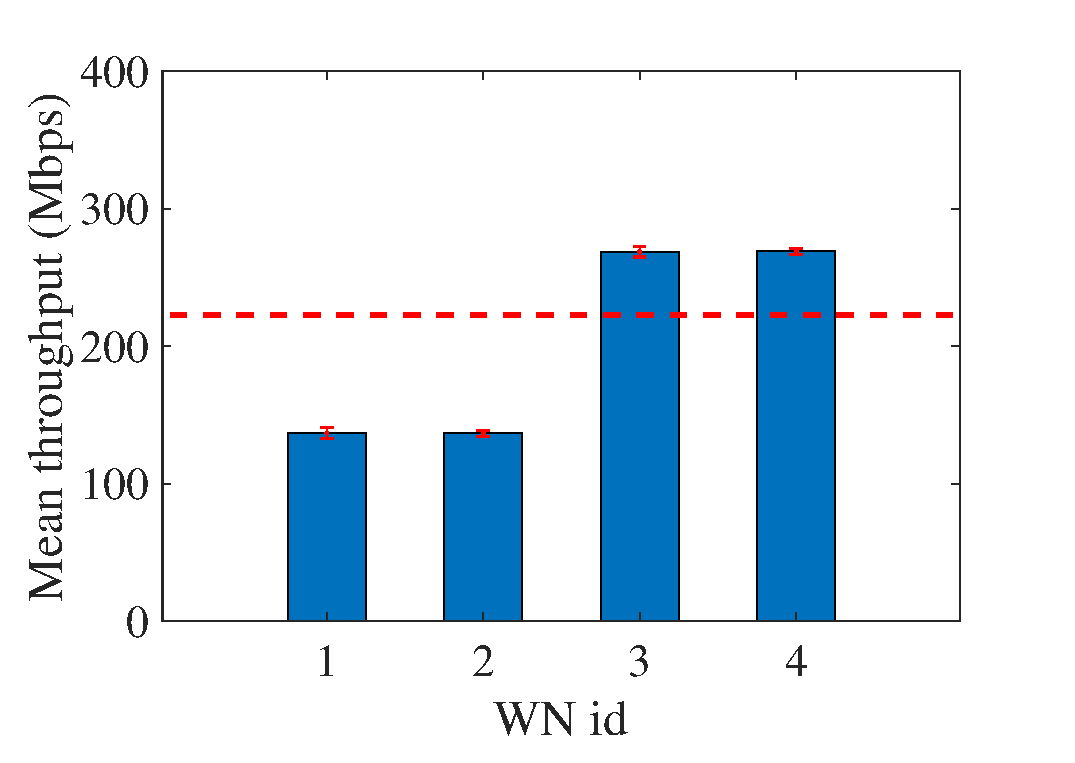
\includegraphics[width=.3\textwidth]{images/NEW_mean_tpt_EXP3_eta1} \\[\abovecaptionskip]
		\small (c) $\eta_0 = 1$
		\label{fig:exp3_eta1_avg_tpt}
	\end{tabular}
	\caption{Average throughput and standard deviation experienced per WN in the last 5,000 iterations of a single EXP3 10000-iterations simulation for different $\eta_0$ values. The proportional fair result is also shown (red dashed line).}
	\label{fig:exp3_avg_tpt}
\end{figure*}

%------------------------
% Study of MAB (UCB)
%------------------------
\subsubsection{Performance of the UCB policy}
\label{section:ucb_study}		
Unlike $\varepsilon$-greedy and EXP3, the basic form of UCB does not include any input parameter to regulate variables such as the learning rate or the exploration coefficient. On the contrary, the action-selection process relies in the generated rewards only. We will study in this section how the previously seen trade-off between fair throughput and variability results for this parameter-free policy.

We start by showing the action probability distribution (shown in Figure \ref{fig:actions_probability_ucb}) derived from the UCB implementation. We observe that WNs clearly prefer playing the actions corresponding to proportional fairness (i.e., the actions with highest transmit power and that result in frequency reuse). 

\begin{figure}[h!]
	\centering							
	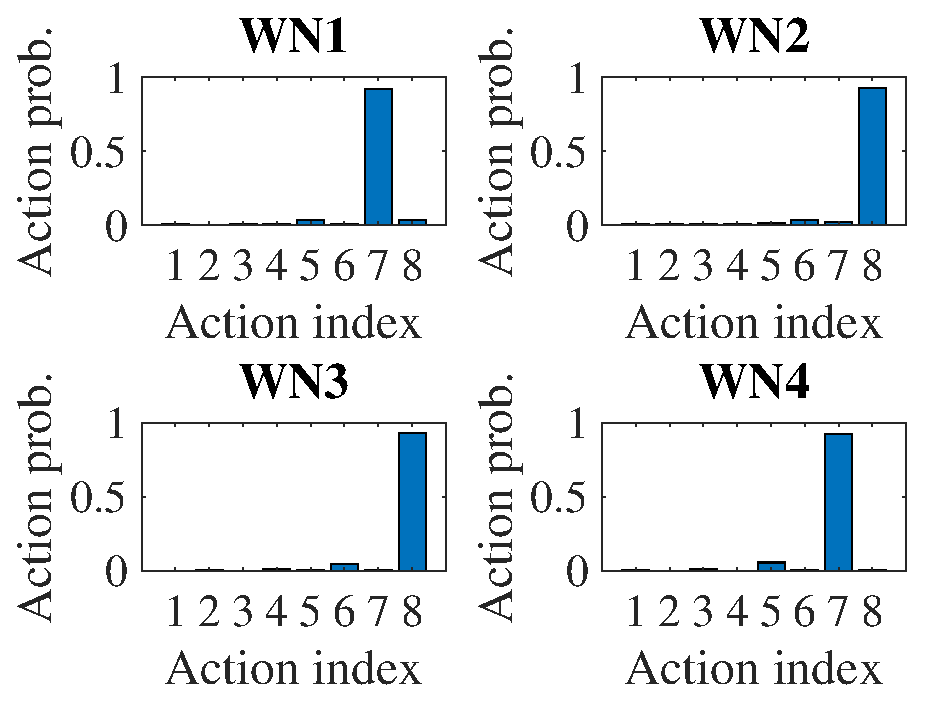
\epsfig{file=images/NEW_actions_probability_UCB.eps, width=6.5cm}
	\caption{Probability of taking a given action in UCB for a simulation of 10,000 iterations.}
	\label{fig:actions_probability_ucb}
\end{figure}	

Now, we concentrate in the temporal aggregate throughput (shown in Figure \ref{fig:ucb_agg_tpt}). The results show a very high variability, which slowly decreases as the number of iterations increases. 
The same observations can be done in the individual throughput evolution (Figure \ref{fig:ucb_tpt_evolution}). As a result, UCB provides long-term fairness but at the expense of a high temporal variability caused by exploration. In Figure \ref{fig:ucb_avg_individual} we show the average throughput experienced by each WN, as well as the standard deviation indicating the suffered variability (only for the last 5,000 iterations). As seen before, one can observe really high fairness but considerable variability due to the temporal evolution of throughput.	

% UCB: aggregate and individual 
\begin{figure*}
	\centering
	\begin{subfigure}[b]{.3\textwidth}
		%\rule{\linewidth}{\linewidth}
		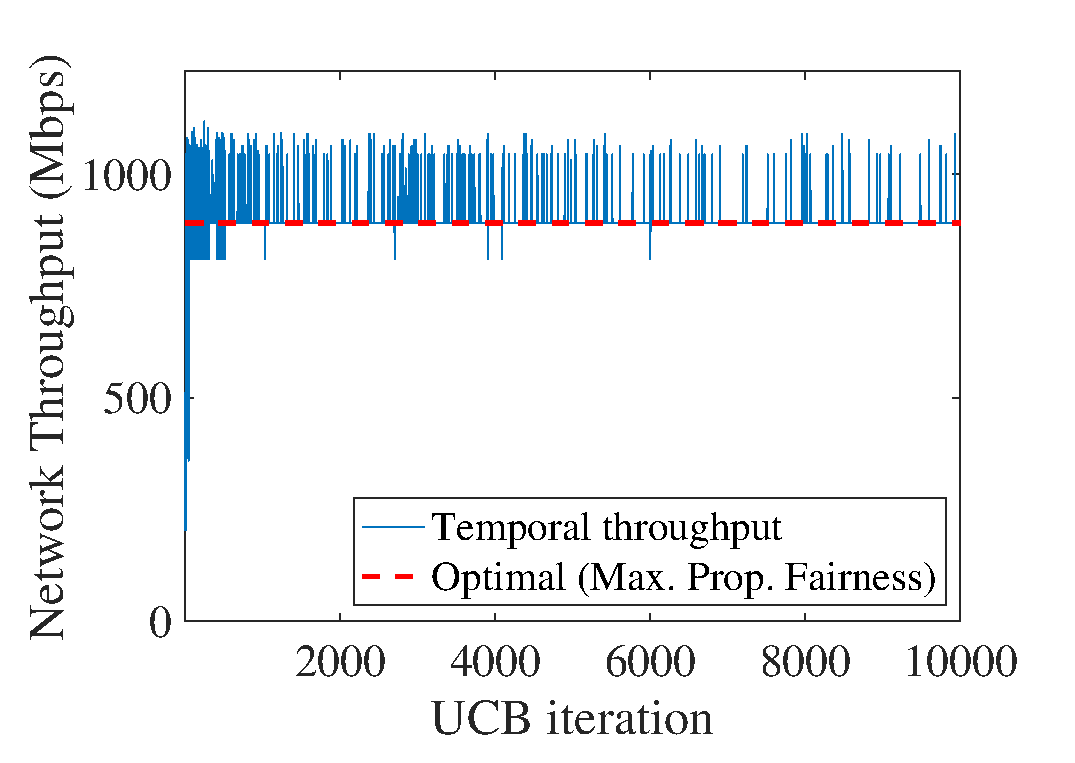
\includegraphics[width=\textwidth]{images/NEW_temporal_aggregate_tpt_UCB}
		\caption{Aggregate}\label{fig:ucb_agg_tpt}
	\end{subfigure}
	\begin{subfigure}[b]{.3\textwidth}
		%\rule{\linewidth}{\linewidth}
		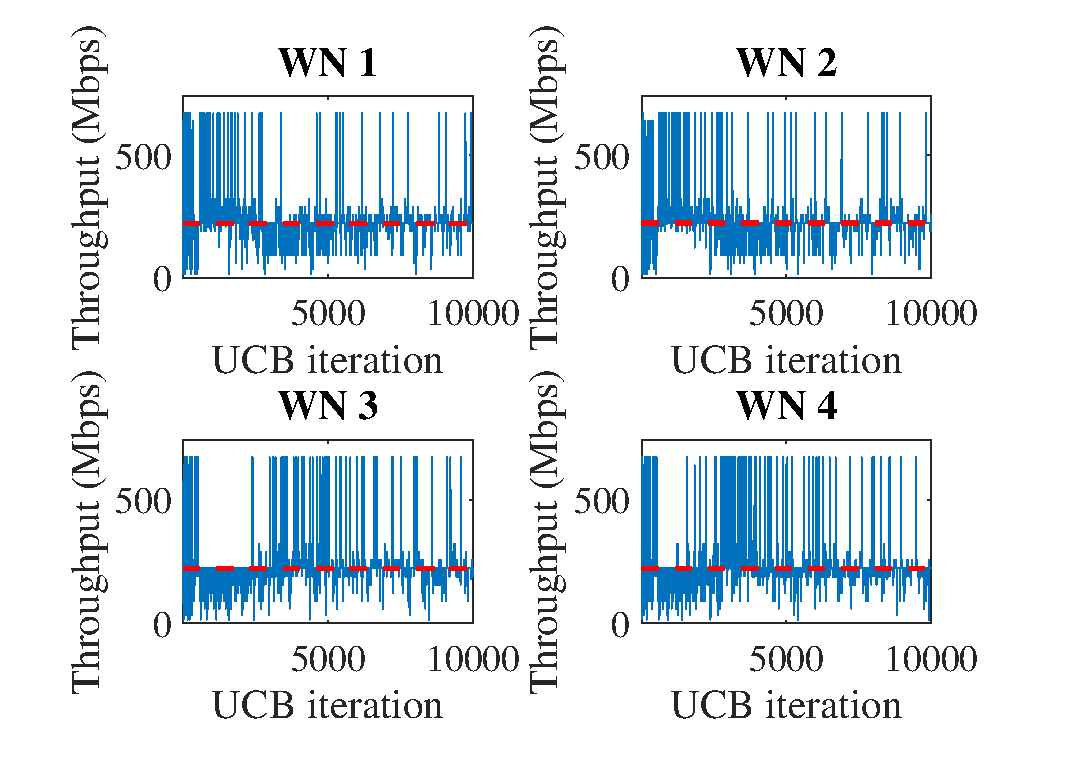
\includegraphics[width=\textwidth]{images/NEW_temporal_individual_tpt_UCB}
		\caption{Individual}\label{fig:ucb_tpt_evolution}
	\end{subfigure}
	\begin{subfigure}[b]{.3\textwidth}
		%\rule{\linewidth}{\linewidth}
		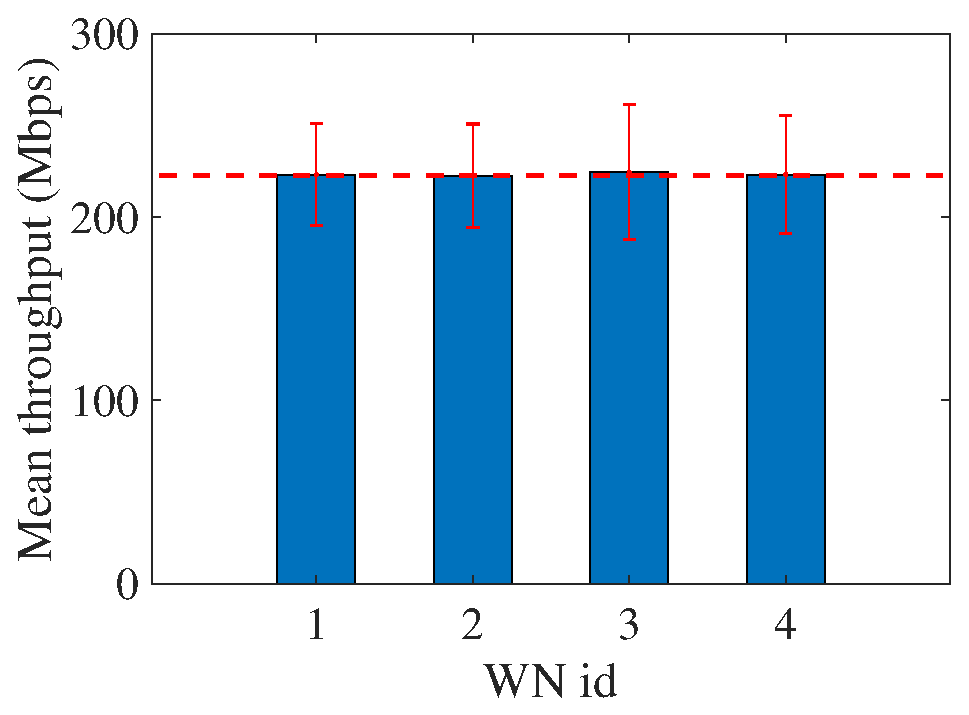
\includegraphics[width=\textwidth]{images/NEW_mean_tpt_UCB}
		\caption{Average}\label{fig:ucb_avg_individual}
	\end{subfigure}
	\caption{Performance achieved for a single UCB 10,000-iterations simulation. The proportional fair result is also shown (red dashed line). (a) Aggregate throughput evolution, (b) Individual throughput evolution, (c) Average individual throughput (the last 5,000 iterations are considered).}
	\label{fig:ucb_tpt}
\end{figure*}

Compared to $\varepsilon$-greedy and EXP3, UCB shows a clearer preference for selecting the proportional fair solutions. However, the intermittent good/poor performance of the actions due to the adversarial setting still keeps the degree of exploration very high, resulting in high temporal variability.

%------------------------
% Study of MAB (TS)
%------------------------
\subsubsection{Performance of the Thompson sampling policy}
\label{section:ts_study}
Similarly to UCB, in the basic form of Thompson sampling we do not have any tunable parameter. As with the other policies, we use a single 10,000-iteration simulation to show in detail the WNs behavior when applying Thompson sampling. We first show the actions probability in Figure \ref{fig:actions_probability_ts}. Note the well-pronounced preference for the proportional fair actions, which indicates fast convergence and little exploratory operations.

% TS: actions probability
\begin{figure}[t!]
	\centering							
	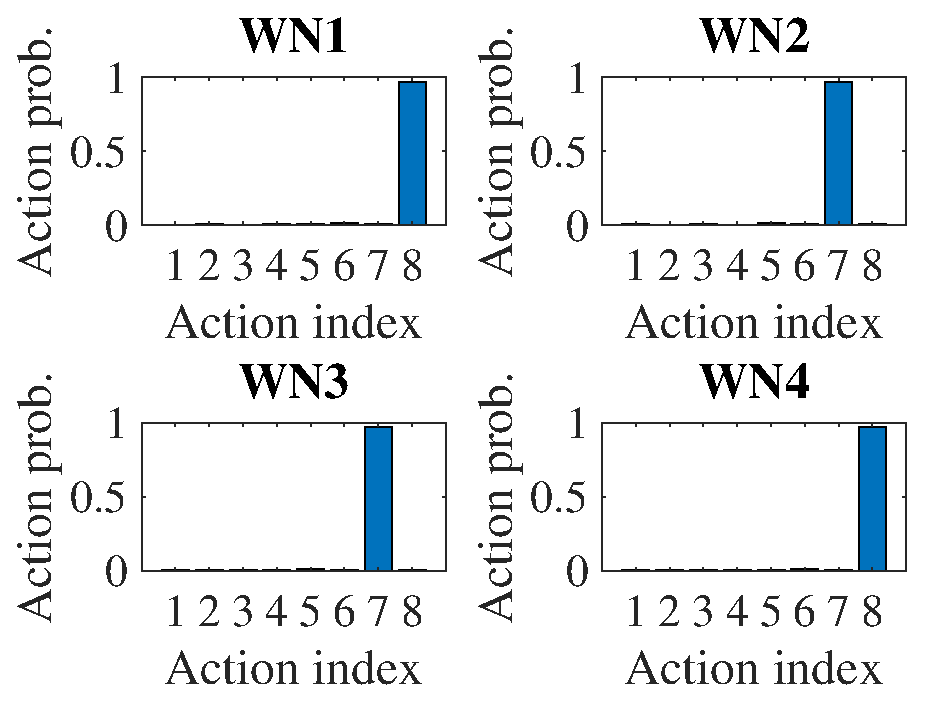
\epsfig{file=images/NEW_actions_probability_TS.eps, width=6.5cm}
	\caption{Probability of taking a given action in Thompson sampling for a simulation of 10,000 iterations.}
	\label{fig:actions_probability_ts}
\end{figure}		

The temporal aggregate throughput is shown in Figure \ref{fig:ts_tpt_evolution}. As it can be observed, Thompson sampling achieves a lower variability in the temporal throughput with respect to UCB. The same observations can be done in the individual throughput evolution (Figure \ref{fig:ts_ind_tpt}). The low temporal variability observed on applying Thompson sampling is highlighted in Figure \ref{fig:ts_avg_individual}, which shows that the average experienced throughput enjoys a low standard deviation. Moreover, high fairness among WNs can be observed.

\begin{figure*}
	\centering
	\begin{subfigure}[b]{.3\textwidth}
		%\rule{\linewidth}{\linewidth}
		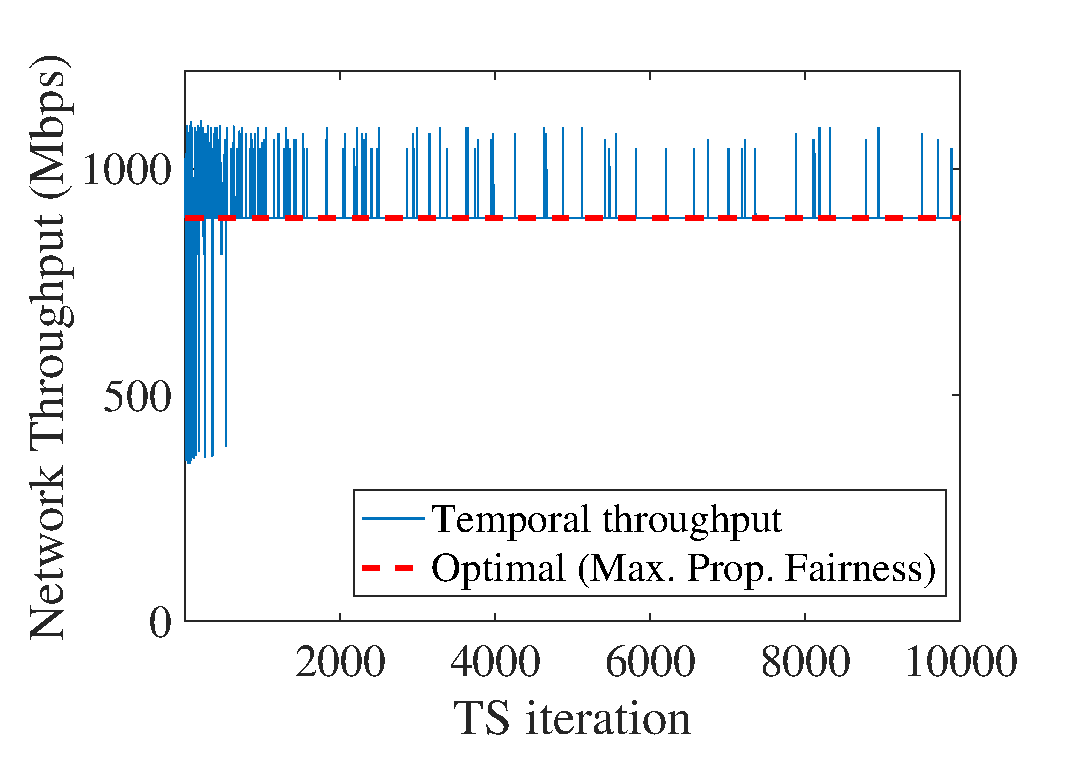
\includegraphics[width=\textwidth]{images/NEW_temporal_aggregate_tpt_TS}
		\caption{Aggregate}\label{fig:ts_agg_tpt}
	\end{subfigure}
	\begin{subfigure}[b]{.3\textwidth}
		%\rule{\linewidth}{\linewidth}
		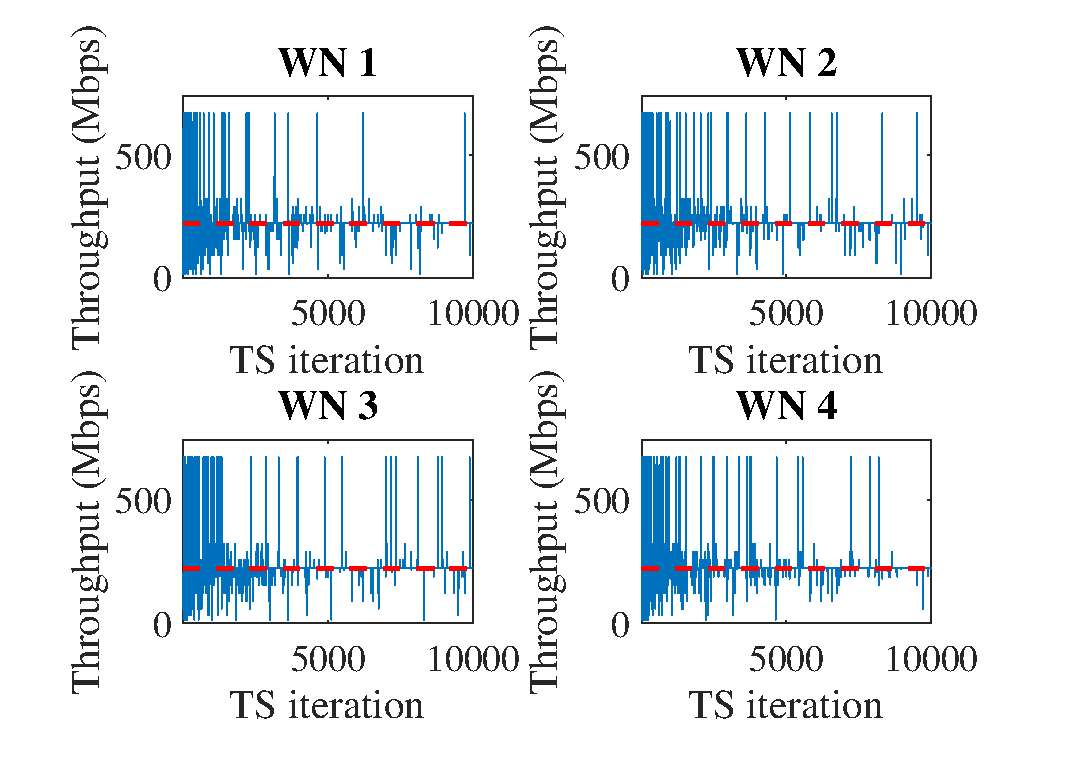
\includegraphics[width=\textwidth]{images/NEW_temporal_individual_tpt_TS}
		\caption{Individual}\label{fig:ts_ind_tpt}
	\end{subfigure}
	\begin{subfigure}[b]{.3\textwidth}
		%\rule{\linewidth}{\linewidth}
		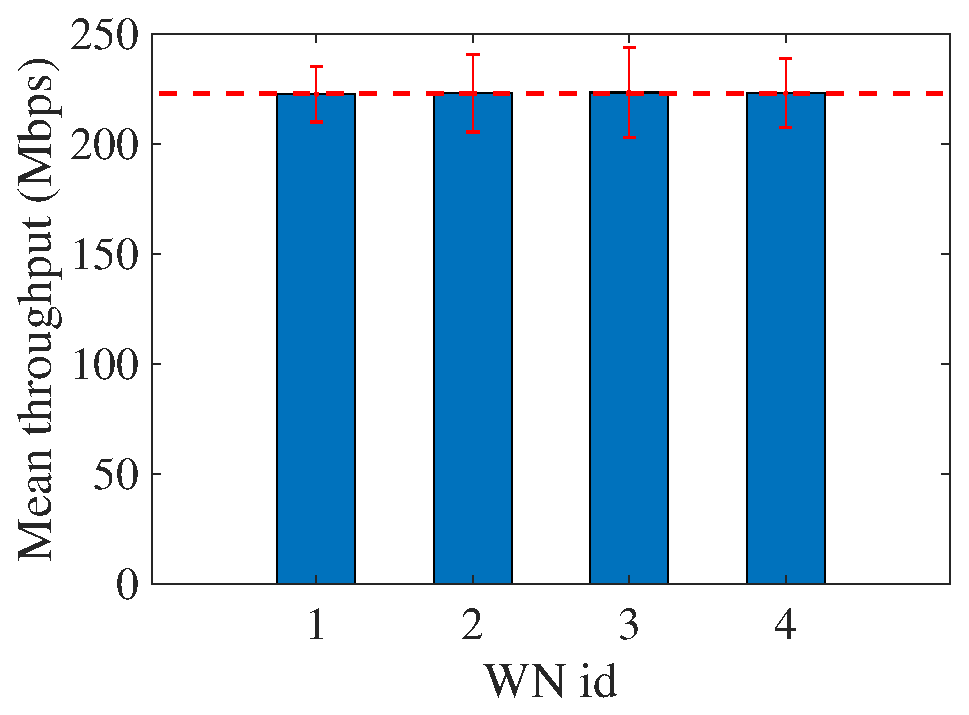
\includegraphics[width=\textwidth]{images/NEW_mean_tpt_TS}
		\caption{Average}\label{fig:ts_avg_individual}
	\end{subfigure}
		\caption{Throughput evolution for a single Thompson sampling 10,000-iterations simulation. The proportional fair result is also shown (red dashed line). (a) Aggregate throughput evolution, (b) Individual throughput evolution, (c) Average individual throughput (the last 5,000 iterations are considered).}
		\label{fig:ts_tpt_evolution}
\end{figure*}

These results show that even though the rewards encourage selfish behavior, the adversarial setting makes Thompson sampling to converge to collaborative actions while keeping the degree of exploration low. Again, this property holds for scenarios where no asymmetries can be found. While the excellent performance we observe echoes other published results that show the superiority of Thompson sampling in various settings \cite{LCLS10}, we highlight that this outstanding empirical performance is actually rather unexpected in our \emph{non-stochastic} setting. Indeed, existing theoretical results only explain the excellent performance of Thompson sampling in \emph{stochastic} bandit problems. On the other hand, the randomization employed by Thompson sampling is at least superficially related to techniques used in game-theoretic online learning \cite{FS97,CBLu06:book}, with the connection made clear only in a special case \cite{Gop13}. The behavior observed in our experiments may indicate a more profound relationship with such game-theoretic algorithms. We leave the investigation of this matter as an exciting direction for future work.

%------------------------
% Random Scenarios - Scalability
%------------------------
\subsection{Random Scenarios}
\label{section:random}
After studying the WNs interactions in the grid scenario, we now evaluate whether the previous conclusions generalize to random scenarios with an arbitrary number of WNs. To this aim, we use the same $10\times5\times 10$ m scenario and randomly allocate $N = \{2, 4, 6, 8\}$ WNs. %Different topologies are captured by placing WNs randomly. With that, we are able to study how the presented policies maintain fairness for different densities and topologies. 

We set $\varepsilon_0 = 1$ in $\varepsilon$-greedy, which is the value that granted the highest aggregate throughput in the experiment shown in Figure \ref{fig:egreedy_tuning_parameters}. We do the same for EXP3 and choose $\eta_0 = 0.6$, which grants the highest aggregate throughput in average (refer to Figure \ref{fig:exp3_tuning_parameters}). In Figure \ref{fig:hist_mean_tpt} we show, for each number of networks and action-selection strategy, an histogram of the mean throughput experienced by each WN during the last 5,000 iterations, and for each of the 100 repetitions.
% Histogram mean throughput
\begin{figure*}
	\centering
	\begin{tabular}{@{}c@{}}
		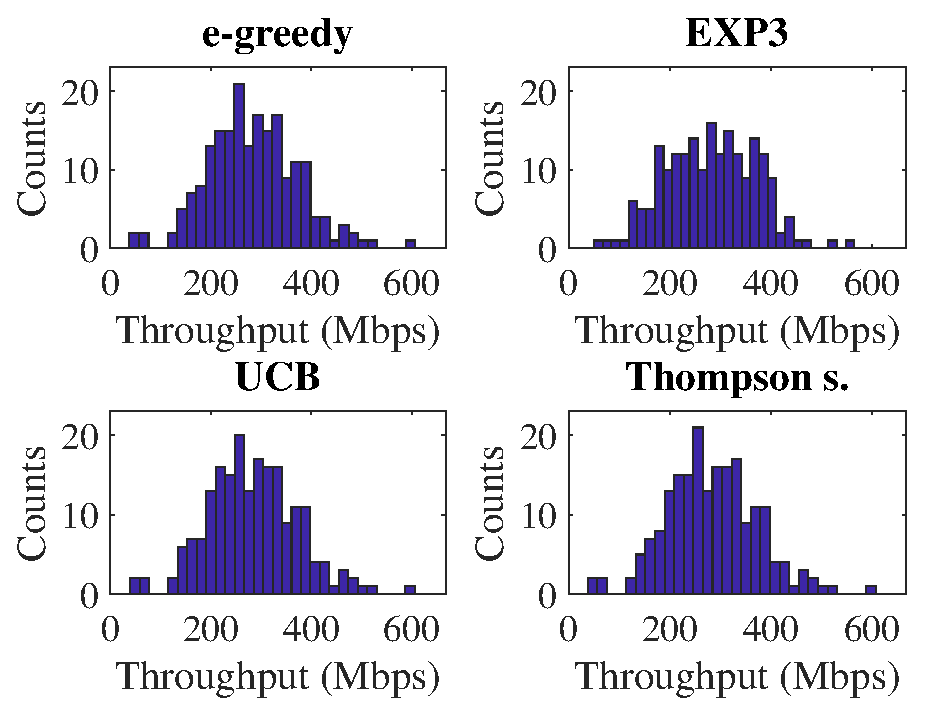
\includegraphics[width=.35\textwidth]{images/hist_mean_tpt_2_WNs} \\[\abovecaptionskip]
		\small (a) N = 2 WNs
		\label{fig:hist_mean_throughput_2}
	\end{tabular}	
	\hspace{\floatsep}	
	\begin{tabular}{@{}c@{}}
		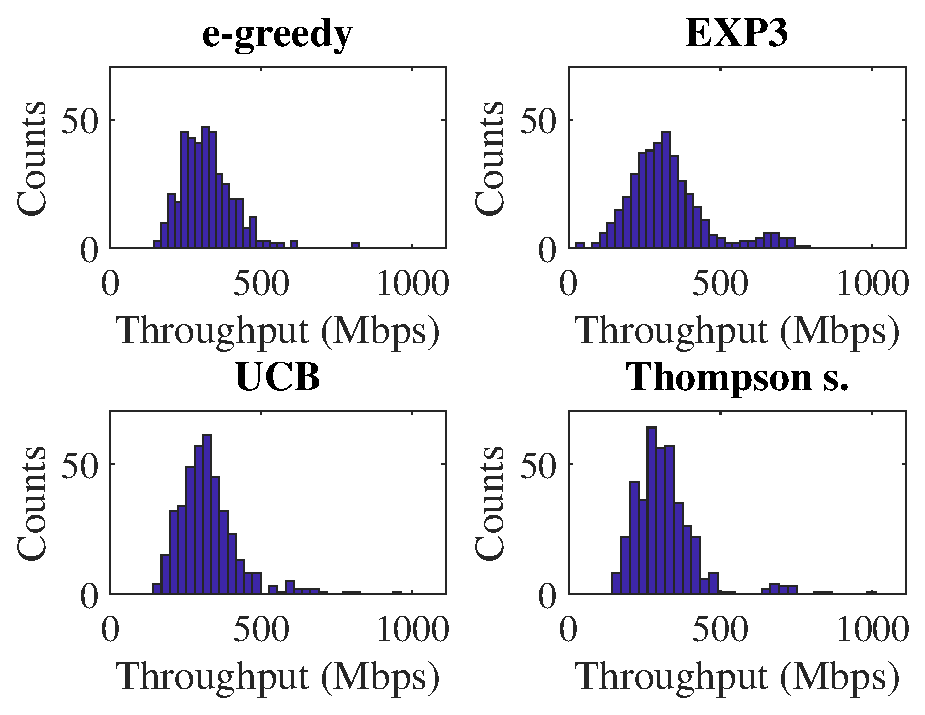
\includegraphics[width=.35\textwidth]{images/hist_mean_tpt_4_WNs} \\[\abovecaptionskip]
		\small (b) N = 4 WNs
		\label{fig:hist_mean_throughput_4}
	\end{tabular}
	\hspace{\floatsep}
	\begin{tabular}{@{}c@{}}
		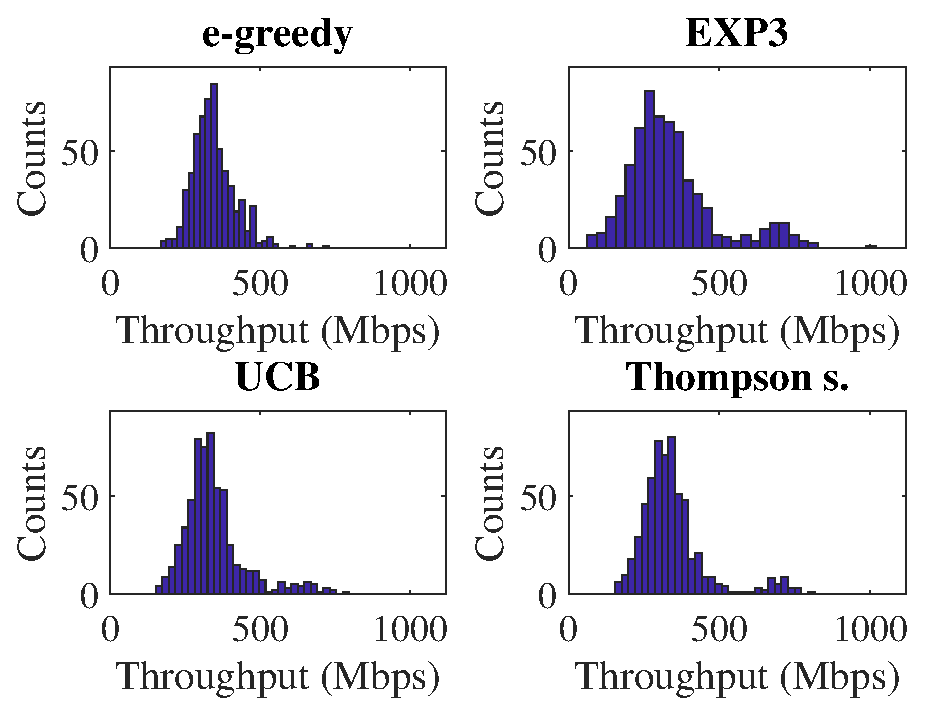
\includegraphics[width=.35\textwidth]{images/hist_mean_tpt_6_WNs} \\[\abovecaptionskip]
		\small (c) N = 6 WNs
		\label{fig:hist_mean_throughput_6}
	\end{tabular}
	\hspace{\floatsep}
	\begin{tabular}{@{}c@{}}
		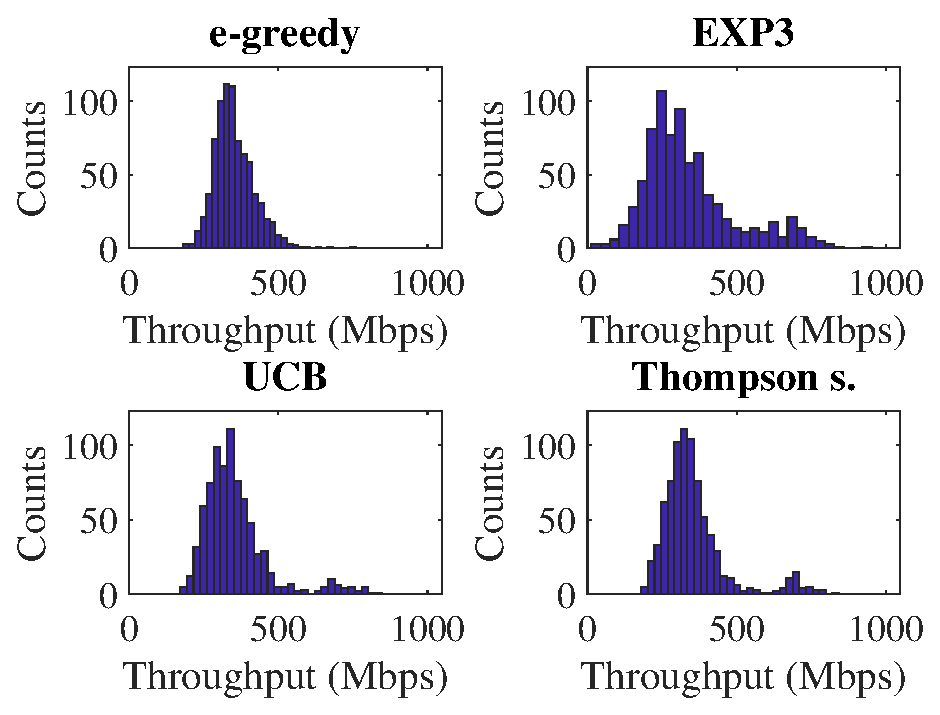
\includegraphics[width=.35\textwidth]{images/hist_mean_tpt_8_WNs} \\[\abovecaptionskip]
		\small (c) N = 8 WNs
		\label{fig:hist_imean_throughput_8}
	\end{tabular}
	\caption{Histogram of the average throughput experienced by each WN during the last 5,000 iterations. Results from 100 repetitions are considered.}
	\label{fig:hist_mean_tpt}
\end{figure*}

As we can observe, histograms of UCB and Thompson sampling are slightly narrower in almost all the cases, which indicates a higher fairness experienced by the WNs with respect to the other policies. Note, as well, that for the $N = 2$, results are similar for all the policies because finding a good-performing configuration in low-density environments is more likely to occur. Thus, fewer exploration is required than for higher densities. Note, as well, that the abovementioned collaborative behavior is still present in random scenarios. In accordance to that, WNs acting selfishly are prone to find a configuration whereby SR is improved in a fair manner. We find the main cause of this issue to be the inter-WN interference sensed at a given transmitter-receiver pair, which is very likely to be similar in both devices for the proposed scenarios. Such a property is given when STAs are close to their associated AP, thus allowing to palliate the effects of asymmetries.

To conclude, we evaluate temporal variability in random scenarios. For that, Table \ref{tbl:std_individual_tpt_experienced} shows the average standard deviation of the throughput experienced by each WN during the last 5,000 iterations (again, we concentrate on the regime after the initial learning phase). We consider the average results from 100 repetitions. With this, we are able to evaluate, for each network density, the variability in the temporal throughput provided by each of the policies in random topologies.
% Mean std of the individual throughput	
\begin{table}[h!]
	\centering
	%\resizebox{\columnwidth}{!}{%
		\begin{tabular}{|c|c|c|c|c|}
			\hline
			\multirow{2}{*}{\textbf{\begin{tabular}[c]{@{}c@{}}Number of \\ WNs\end{tabular}}} & \multicolumn{4}{c|}{\textbf{$\overline{\sigma}(\Gamma_{i \in N})$ (Mbps)}} \\ \cline{2-5} 
			& \textbf{$\varepsilon$-greedy} & \textbf{EXP3} & \textbf{UCB} & \textbf{Thompson s.} \\ \hline
			\textbf{2} & 12.1314 & 31.2897 & 31.9422 & 12.2079 \\ \hline
			\textbf{4} & 83.7318 & 95.4976 & 73.9136 & 50.6985 \\ \hline
			\textbf{6} & 120.8570 & 81.3259 & 67.6045 & 62.8171 \\ \hline
			\textbf{8} & 130.0322 & 73.5171 & 63.2272 & 68.8547 \\ \hline
	\end{tabular}%}
	\caption{Mean standard deviation of the throughput experienced $\Gamma_{i \in N}$ by each $WN_i$ during the last 5,000 iterations. 100 repetitions are considered for averaging purposes.}
	\label{tbl:std_individual_tpt_experienced}
\end{table}	

As previously seen in the toy grid scenario introduced in Section \ref{section:toy_grid_scenario}, both UCB and Thompson sampling provide the best results in terms of temporal throughput variability. Despite $\varepsilon$-greedy provides very good results for $N=2$, it does not properly scale up with the number of WNs.   

%%%%%%%%%%%%%%%
%  VI. CONCLUSIONS  %
%%%%%%%%%%%%%%%
\section{Conclusions }
\label{section:conclusions}
In this paper, we provided a tutorial-like implementation of MABs to address the decentralized SR problem in dense WNs. Unlike previous literature, we have focused on a situation in which few resources are available, thus bringing out the competition issues raised from the adversarial setting. Our results show that decentralized learning allows improving SR in dense WN, so that collaborative results in symmetric scenarios, sometimes close to optimal proportional fairness, can be achieved. This result is achieved even though WNs act selfishly, aiming to maximize their own throughput. In addition, this behavior is observed for random scenarios, where the effects of asymmetries cannot be controlled. %However, using only local information in limited resources scenarios conducts to an adversarial setting in which a pure strategy does not exist, which prevents reaching a Nash Equilibrium. In the WNs case, applying decentralized learning in such an adversarial setting entails noticing a high temporal variability in the experienced throughput. 
These collaborative actions are, at times, accompanied by high temporal throughput variability, which can be understood as a consequence of the  rate at which networks change their configuration in response of the opponents behavior. A high temporal variability may provoke negative issues in a node's performance, as its effects may be propagated to higher layers of the protocol stack. For instance, a high throughput fluctuation may entail behavioral anomalies in protocols such as Transmission Control Protocol (TCP). %In this case, the temporal fluctuation of the throughput would directly affect the Contention Window (CW) used in TCP for congestion control, providing a poor performance. 
We have studied this trade-off between fair resource allocation and high temporal throughput variability in $\varepsilon$-greedy, EXP3, UCB and Thompson sampling action-selection strategies. Our results show that while this trade-off is hard to regulate via the learning parameters in $\varepsilon$-greedy and EXP3, UCB  and, especially, Thompson sampling are able to achieve fairness at a reduced temporal variability. We identify the root cause of this phenomena to the fact that both UCB and Thompson sampling consider the probability distribution of the rewards, and not only their magnitude.

We left as future work to further study the MABs application to WNs through distributed (with message passing) and centralized (with complete information) approaches with shared reward. Furthermore, we would like to extend this work to enhance both throughput and stability by inferring the actions of the opponents and acting in consequence. Defining the resource allocation problem as an adversarial game is one possibility to do so. Finally, we intend to particularize to IEEE 802.11 WLANs to study the effects of applying RL when using a medium access protocol such as CSMA. In fact, this would let us consider dynamic Carrier Sense Threshold (CST) to further enable SR.

%%%%%%%%%%%%%%%%%%%%%%%%%
%%%  ACKNOWLEDGEMENT  		  %%%
%%%%%%%%%%%%%%%%%%%%%%%%%
% use section* for acknowledgment
% The Computer Society usually uses the plural form
\section*{Acknowledgments}
This work has been partially supported by the Spanish Ministry of Economy and Competitiveness under the Maria de Maeztu Units of Excellence Programme (MDM-2015-0502), by the European Regional Development Fund under grant TEC2015-71303-R (MINECO/FEDER), and by a Gift from CISCO University Research Program (CG\#890107) \& Silicon Valley Community Foundation.

%%%%%%%%%%%%%%%%%%%%%%%%%
%%%  BIBLIOGRAPHY    
%%%%%%%%%%%%%%%%%%%%%%%%%
\newpage
\bibliographystyle{unsrt}
\bibliography{references}

\end{document}